%%
%% This is file `sample-manuscript.tex',
%% generated with the docstrip utility.
%%
%% The original source files were:
%%
%% samples.dtx  (with options: `all,proceedings,bibtex,manuscript')
%% 
%% IMPORTANT NOTICE:
%% 
%% For the copyright see the source file.
%% 
%% Any modified versions of this file must be renamed
%% with new filenames distinct from sample-manuscript.tex.
%% 
%% For distribution of the original source see the terms
%% for copying and modification in the file samples.dtx.
%% 
%% This generated file may be distributed as long as the
%% original source files, as listed above, are part of the
%% same distribution. (The sources need not necessarily be
%% in the same archive or directory.)
%%
%%
%% Commands for TeXCount
%TC:macro \cite [option:text,text]
%TC:macro \citep [option:text,text]
%TC:macro \citet [option:text,text]
%TC:envir table 0 1
%TC:envir table* 0 1
%TC:envir tabular [ignore] word
%TC:envir displaymath 0 word
%TC:envir math 0 word
%TC:envir comment 0 0
%%
%%
%% The first command in your LaTeX source must be the \documentclass
%% command.
%%
%% For submission and review of your manuscript please change the
%% command to \documentclass[manuscript, screen, review]{acmart}.
%%
%% When submitting camera ready or to TAPS, please change the command
%% to \documentclass[sigconf]{acmart} or whichever template is required
%% for your publication.
%%
%%
% \documentclass[manuscript,screen,review, anonymous]{acmart}
% \documentclass[manuscript,review,screen,anonymous]{acmart}
\documentclass[sigconf,screen]{acmart}

%%
%% \BibTeX command to typeset BibTeX logo in the docs
\AtBeginDocument{%
  \providecommand\BibTeX{{%
    acmart\TeX}}}

%% Rights management information.  This information is sent to you
%% when you complete the rights form.  These commands have SAMPLE
%% values in them; it is your responsibility as an author to replace
%% the commands and values with those provided to you when you
%% complete the rights form.

\copyrightyear{2025}
\acmYear{2025}
\setcopyright{cc}
\setcctype{by-nc-sa}
\acmConference[CHI '25]{CHI Conference on Human Factors in Computing Systems}{April 26-May 1, 2025}{Yokohama, Japan}
\acmBooktitle{CHI Conference on Human Factors in Computing Systems (CHI '25), April 26-May 1, 2025, Yokohama, Japan}\acmDOI{10.1145/3706598.3714104}
\acmISBN{979-8-4007-1394-1/25/04}

%% These commands are for a PROCEEDINGS abstract or paper.
\acmConference[Conference acronym 'XX]{Make sure to enter the correct
  conference title from your rights confirmation emai}{June 03--05,
  2018}{Woodstock, NY}
%%
%%  Uncomment \acmBooktitle if the title of the proceedings is different
%%  from ``Proceedings of ...''!
%%
%%\acmBooktitle{Woodstock '18: ACM Symposium on Neural Gaze Detection,
%%  June 03--05, 2018, Woodstock, NY}
% \acmISBN{978-1-4503-XXXX-X/18/06}


%%
%% end of the preamble, start of the body of the document source.
% \citestyle{acmauthoryear}

\graphicspath{{figures/}{pictures/}{images/}{./}} % where to search for the images

\usepackage{algorithm}
\renewcommand{\figurename}{Figure}
\usepackage{color}
\usepackage{enumitem}
\usepackage{xspace}
\usepackage{listings}

\newcommand{\ie}{{i.e.,}\xspace}
\newcommand{\eg}{{e.g.,}\xspace}
\newcommand{\ea}{{et~al.}\xspace}
\newcommand{\etal}{{et~al.}\xspace}
\newcommand{\aka}{{a.k.a.}\xspace}
\newcommand{\etc}{{etc\xperiod}\xspace}
\newcommand{\f}[1]{{\color{black} #1}}
\newcommand{\g}[1]{{\color{black} #1}}
\newcommand{\re}[1]{{\color{black} #1}}
\newcommand{\cp}[1]{{\color{RoyalBlue} #1}}
% \newcommand{\att}[1]{{\color{BrickRed} #1}}
\newcommand{\red}[1]{{\color{Red} #1}}
\newcommand{\todo}[1]{{\color{orange} todo: #1}}
\definecolor{bluecrayola}{rgb}{0.12,0.46,1.0}
\renewcommand{\ttdefault}{txtt}

\newcommand{\argu}[1]{\texttt{\emph{#1}}}

\newcommand{\sop}[1]{{\color{cop} \texttt{#1}}}
\newcommand{\sobj}[1]{{\color{cobj} \texttt{#1}}}
\newcommand{\spar}[1]{{\color{cpar} \texttt{#1}}}

\newcommand{\sact}[3]{\texttt{\{\sop{#1}, \sobj{#2}, \spar{#3}\}}}
\newcommand{\sutt}[1]{{\color{cutt} ``#1''}}
\newcommand{\copied}[1]{{\color{gray}\textit{[Placeholder: #1]}}}

\newcommand{\tool}{InterLink\xspace}

\definecolor{mygreen}{RGB}{0,176,80}
\definecolor{mygreen2}{RGB}{232, 245, 233}
\definecolor{myorange}{RGB}{192, 0, 0}
\definecolor{myblue}{RGB}{47, 85, 151}
\newcommand{\highlightone}[1]{\colorbox{mygreen2}{\textcolor{mygreen}{#1}}}
\newcommand{\highlighttwo}[1]{\colorbox{myblue}{\textcolor{white}{#1}}}

\newcommand{\yanna}[1]{{\color{black} {#1}}}
% \newcommand{\reviewerCom}[1]{{\color{blue} {#1}}}
% \newcommand{\review}[1]{\textcolor{purple}{#1}}
\newcommand{\concise}[1]{\textcolor{black}{#1}}

\newcommand{\revise}[1]{{\color{black} {#1}}}
\newcommand{\reviewerCom}[1]{{\color{black} {#1}}}
\newcommand{\review}[1]{\textcolor{black}{}}

\newcommand{\final}[1]{{\color{black} {#1}}}

\renewcommand{\sectionautorefname}{Section}
\renewcommand{\subsectionautorefname}{Section}
\renewcommand{\subsubsectionautorefname}{Section}

% \documentclass{article}





\begin{document}

\title{InterLink: Linking Text with Code and Output in Computational Notebooks}

\lstset{
    basicstyle=\ttfamily\small, % Use a small true type font for code
    keywordstyle=\color{blue}, % Set specific colors for components (optional)
    identifierstyle=\color{black},
    commentstyle=\color{green},
    stringstyle=\color{red},
    frame=single, % Frame around the code block
    breaklines=true, % Automatic line breaking
    showstringspaces=false, % Don't show spaces in strings as special character
    tabsize=2, % Sets default tabsize to 2 spaces
    captionpos=b % Sets the caption-position to bottom
}


%%
%% The "author" command and its associated commands are used to define
%% the authors and their affiliations.
%% Of note is the shared affiliation of the first two authors, and the
%% "authornote" and "authornotemark" commands
%% used to denote shared contribution to the research.


\author{Yanna Lin}
\authornote{The work was done when Yanna Lin was visiting CMU.}
\orcid{0000-0003-3730-0827}
\affiliation{%
  \institution{The Hong Kong University of Science and Technology}
  \city{Hong Kong SAR}
  \country{China}
}
\affiliation{%
  \institution{Carnegie Mellon University}
  \city{Pittsburgh, PA}
  \country{United States}
}
\email{ylindg@connect.ust.hk}

\author{Leni Yang}
% \authornote{The work was done when Haotian Li was in HKUST.}
\orcid{0000-0003-4527-4905}
\affiliation{%
  \institution{The Hong Kong University of Science and Technology}
  \city{Hong Kong SAR}
  \country{China}
}
\email{lyangbb@connect.ust.hk}



\author{Haotian Li}
\authornote{The work was done when Haotian Li was at HKUST.}
\orcid{0000-0001-9547-3449}
\affiliation{%
  \institution{Microsoft Research Asia}
  \city{Beijing}
  \country{China}
}
\email{haotian.li@microsoft.com}


\author{Huamin Qu}
% \authornote{The work was done when Haotian Li was in HKUST.}
\orcid{0000-0002-3344-9694}
\affiliation{%
  \institution{The Hong Kong University of Science and Technology}
  \city{Hong Kong SAR}
  \country{China}
}
\email{huamin@cse.ust.hk}

\author{Dominik Moritz}
\authornote{Dominik Moritz is the corresponding author.}
\orcid{0000-0002-3110-1053}
\affiliation{%
  \institution{Carnegie Mellon University}
  \city{Pittsburgh, PA}
  \country{United States}
}
\email{domoritz@cmu.edu}

% \author{Ben Trovato}
% \authornote{Both authors contributed equally to this research.}
% \orcid{1234-5678-9012}
% \author{G.K.M. Tobin}
% \authornotemark[1]
% \email{webmaster@marysville-ohio.com}
% \affiliation{%
%   \institution{Institute for Clarity in Documentation}
%   \city{Dublin}
%   \state{Ohio}
%   \country{USA}
% }


%% By default, the full list of authors will be used in the page
%% headers. Often, this list is too long, and will overlap
%% other information printed in the page headers. This command allows
%% the author to define a more concise list
%% of authors' names for this purpose.
% \renewcommand{\shortauthors}{Trovato et al.
%%
%% The abstract is a short summary of the work to be presented in the
%% article.
\begin{abstract}
\begin{abstract}  
Test time scaling is currently one of the most active research areas that shows promise after training time scaling has reached its limits.
Deep-thinking (DT) models are a class of recurrent models that can perform easy-to-hard generalization by assigning more compute to harder test samples.
However, due to their inability to determine the complexity of a test sample, DT models have to use a large amount of computation for both easy and hard test samples.
Excessive test time computation is wasteful and can cause the ``overthinking'' problem where more test time computation leads to worse results.
In this paper, we introduce a test time training method for determining the optimal amount of computation needed for each sample during test time.
We also propose Conv-LiGRU, a novel recurrent architecture for efficient and robust visual reasoning. 
Extensive experiments demonstrate that Conv-LiGRU is more stable than DT, effectively mitigates the ``overthinking'' phenomenon, and achieves superior accuracy.
\end{abstract}  
\end{abstract}

\begin{teaserfigure}
  \includegraphics[width=\linewidth,alt={Composite figure showing user frustration with a traditional long, linear notebook on the left, and an innovative side-by-side layout of our system on the right. The left side depicts a notebook with dense text and graphics, overlayed with a user's thought bubble expressing difficulty in locating information due to the notebook's complexity. The right side shows our system's interface with observations noted on the left pane and corresponding code and outputs on the right pane, simplifying data navigation and linking results directly to their source code. 
  }]{figures/teaser0.1_shorter.png}
  \caption{
  \tool helps analysts read and understand computational notebooks by linking text to code and outputs using a side-by-side layout.
  Clicking the icon in the toolbar (b1) activates \tool, switching the layout of the notebook from a linear layout (A) to a side-by-side layout (B).
  In (B), the ``observation'' cell, marked with the fixed icon (b2), indicates that it has been fixed in place through a click, ensuring it remains visible on the screen for easy reference.
  A linking line (b3) explicitly connects the ``observation'' cell to the code cell (b4).
  Visual cues (b5-b7), including colored underlines, dashed borders, and dashed sketches, indicate the existence of relationships between segments or cells.
}
    \Description{Composite figure showing user frustration with a traditional long, linear notebook on the left, and an innovative side-by-side layout of our system on the right. The left side depicts a notebook with dense text and graphics, overlayed with a user's thought bubble expressing difficulty in locating information due to the notebook's complexity. The right side shows our system's interface with observations noted on the left pane and corresponding code and outputs on the right pane, simplifying data navigation and linking results directly to their source code. }
  \label{fig: teaser}
\end{teaserfigure}

%%
%% The code below is generated by the tool at http://dl.acm.org/ccs.cfm.
%% Please copy and paste the code instead of the example below.
%%

\begin{CCSXML}
<ccs2012>
   <concept>
       <concept_id>10003120.10003121.10003124.10010865</concept_id>
       <concept_desc>Human-centered computing~Graphical user interfaces</concept_desc>
       <concept_significance>500</concept_significance>
       </concept>
 </ccs2012>
\end{CCSXML}

\ccsdesc[500]{Human-centered computing~Graphical user interfaces}

%%
%% Keywords. The author(s) should pick words that accurately describe
%% the work being presented. Separate the keywords with commas.
\keywords{Computational Notebook, User Comprehension, Text-Code/Output Linking, Interactive Computational Notebook}

% \received{20 February 2007}
% \received[revised]{12 March 2009}
% \received[accepted]{5 June 2009}

%%
%% This command processes the author and affiliation and title
%% information and builds the first part of the formatted document.
\maketitle


\section{Introduction}
\label{sec:introduction}
The business processes of organizations are experiencing ever-increasing complexity due to the large amount of data, high number of users, and high-tech devices involved \cite{martin2021pmopportunitieschallenges, beerepoot2023biggestbpmproblems}. This complexity may cause business processes to deviate from normal control flow due to unforeseen and disruptive anomalies \cite{adams2023proceddsriftdetection}. These control-flow anomalies manifest as unknown, skipped, and wrongly-ordered activities in the traces of event logs monitored from the execution of business processes \cite{ko2023adsystematicreview}. For the sake of clarity, let us consider an illustrative example of such anomalies. Figure \ref{FP_ANOMALIES} shows a so-called event log footprint, which captures the control flow relations of four activities of a hypothetical event log. In particular, this footprint captures the control-flow relations between activities \texttt{a}, \texttt{b}, \texttt{c} and \texttt{d}. These are the causal ($\rightarrow$) relation, concurrent ($\parallel$) relation, and other ($\#$) relations such as exclusivity or non-local dependency \cite{aalst2022pmhandbook}. In addition, on the right are six traces, of which five exhibit skipped, wrongly-ordered and unknown control-flow anomalies. For example, $\langle$\texttt{a b d}$\rangle$ has a skipped activity, which is \texttt{c}. Because of this skipped activity, the control-flow relation \texttt{b}$\,\#\,$\texttt{d} is violated, since \texttt{d} directly follows \texttt{b} in the anomalous trace.
\begin{figure}[!t]
\centering
\includegraphics[width=0.9\columnwidth]{images/FP_ANOMALIES.png}
\caption{An example event log footprint with six traces, of which five exhibit control-flow anomalies.}
\label{FP_ANOMALIES}
\end{figure}

\subsection{Control-flow anomaly detection}
Control-flow anomaly detection techniques aim to characterize the normal control flow from event logs and verify whether these deviations occur in new event logs \cite{ko2023adsystematicreview}. To develop control-flow anomaly detection techniques, \revision{process mining} has seen widespread adoption owing to process discovery and \revision{conformance checking}. On the one hand, process discovery is a set of algorithms that encode control-flow relations as a set of model elements and constraints according to a given modeling formalism \cite{aalst2022pmhandbook}; hereafter, we refer to the Petri net, a widespread modeling formalism. On the other hand, \revision{conformance checking} is an explainable set of algorithms that allows linking any deviations with the reference Petri net and providing the fitness measure, namely a measure of how much the Petri net fits the new event log \cite{aalst2022pmhandbook}. Many control-flow anomaly detection techniques based on \revision{conformance checking} (hereafter, \revision{conformance checking}-based techniques) use the fitness measure to determine whether an event log is anomalous \cite{bezerra2009pmad, bezerra2013adlogspais, myers2018icsadpm, pecchia2020applicationfailuresanalysispm}. 

The scientific literature also includes many \revision{conformance checking}-independent techniques for control-flow anomaly detection that combine specific types of trace encodings with machine/deep learning \cite{ko2023adsystematicreview, tavares2023pmtraceencoding}. Whereas these techniques are very effective, their explainability is challenging due to both the type of trace encoding employed and the machine/deep learning model used \cite{rawal2022trustworthyaiadvances,li2023explainablead}. Hence, in the following, we focus on the shortcomings of \revision{conformance checking}-based techniques to investigate whether it is possible to support the development of competitive control-flow anomaly detection techniques while maintaining the explainable nature of \revision{conformance checking}.
\begin{figure}[!t]
\centering
\includegraphics[width=\columnwidth]{images/HIGH_LEVEL_VIEW.png}
\caption{A high-level view of the proposed framework for combining \revision{process mining}-based feature extraction with dimensionality reduction for control-flow anomaly detection.}
\label{HIGH_LEVEL_VIEW}
\end{figure}

\subsection{Shortcomings of \revision{conformance checking}-based techniques}
Unfortunately, the detection effectiveness of \revision{conformance checking}-based techniques is affected by noisy data and low-quality Petri nets, which may be due to human errors in the modeling process or representational bias of process discovery algorithms \cite{bezerra2013adlogspais, pecchia2020applicationfailuresanalysispm, aalst2016pm}. Specifically, on the one hand, noisy data may introduce infrequent and deceptive control-flow relations that may result in inconsistent fitness measures, whereas, on the other hand, checking event logs against a low-quality Petri net could lead to an unreliable distribution of fitness measures. Nonetheless, such Petri nets can still be used as references to obtain insightful information for \revision{process mining}-based feature extraction, supporting the development of competitive and explainable \revision{conformance checking}-based techniques for control-flow anomaly detection despite the problems above. For example, a few works outline that token-based \revision{conformance checking} can be used for \revision{process mining}-based feature extraction to build tabular data and develop effective \revision{conformance checking}-based techniques for control-flow anomaly detection \cite{singh2022lapmsh, debenedictis2023dtadiiot}. However, to the best of our knowledge, the scientific literature lacks a structured proposal for \revision{process mining}-based feature extraction using the state-of-the-art \revision{conformance checking} variant, namely alignment-based \revision{conformance checking}.

\subsection{Contributions}
We propose a novel \revision{process mining}-based feature extraction approach with alignment-based \revision{conformance checking}. This variant aligns the deviating control flow with a reference Petri net; the resulting alignment can be inspected to extract additional statistics such as the number of times a given activity caused mismatches \cite{aalst2022pmhandbook}. We integrate this approach into a flexible and explainable framework for developing techniques for control-flow anomaly detection. The framework combines \revision{process mining}-based feature extraction and dimensionality reduction to handle high-dimensional feature sets, achieve detection effectiveness, and support explainability. Notably, in addition to our proposed \revision{process mining}-based feature extraction approach, the framework allows employing other approaches, enabling a fair comparison of multiple \revision{conformance checking}-based and \revision{conformance checking}-independent techniques for control-flow anomaly detection. Figure \ref{HIGH_LEVEL_VIEW} shows a high-level view of the framework. Business processes are monitored, and event logs obtained from the database of information systems. Subsequently, \revision{process mining}-based feature extraction is applied to these event logs and tabular data input to dimensionality reduction to identify control-flow anomalies. We apply several \revision{conformance checking}-based and \revision{conformance checking}-independent framework techniques to publicly available datasets, simulated data of a case study from railways, and real-world data of a case study from healthcare. We show that the framework techniques implementing our approach outperform the baseline \revision{conformance checking}-based techniques while maintaining the explainable nature of \revision{conformance checking}.

In summary, the contributions of this paper are as follows.
\begin{itemize}
    \item{
        A novel \revision{process mining}-based feature extraction approach to support the development of competitive and explainable \revision{conformance checking}-based techniques for control-flow anomaly detection.
    }
    \item{
        A flexible and explainable framework for developing techniques for control-flow anomaly detection using \revision{process mining}-based feature extraction and dimensionality reduction.
    }
    \item{
        Application to synthetic and real-world datasets of several \revision{conformance checking}-based and \revision{conformance checking}-independent framework techniques, evaluating their detection effectiveness and explainability.
    }
\end{itemize}

The rest of the paper is organized as follows.
\begin{itemize}
    \item Section \ref{sec:related_work} reviews the existing techniques for control-flow anomaly detection, categorizing them into \revision{conformance checking}-based and \revision{conformance checking}-independent techniques.
    \item Section \ref{sec:abccfe} provides the preliminaries of \revision{process mining} to establish the notation used throughout the paper, and delves into the details of the proposed \revision{process mining}-based feature extraction approach with alignment-based \revision{conformance checking}.
    \item Section \ref{sec:framework} describes the framework for developing \revision{conformance checking}-based and \revision{conformance checking}-independent techniques for control-flow anomaly detection that combine \revision{process mining}-based feature extraction and dimensionality reduction.
    \item Section \ref{sec:evaluation} presents the experiments conducted with multiple framework and baseline techniques using data from publicly available datasets and case studies.
    \item Section \ref{sec:conclusions} draws the conclusions and presents future work.
\end{itemize}

%\section{Related Work}
%\label{sec:related-work}

%\subsection{Background}

%Defect detection is critical to ensure the yield of integrated circuit manufacturing lines and reduce faults. Previous research has primarily focused on wafer map data, which engineers produce by marking faulty chips with different colors based on test results. The specific spatial distribution of defects on a wafer can provide insights into the causes, thereby helping to determine which stage of the manufacturing process is responsible for the issues. Although such research is relatively mature, the continual miniaturization of integrated circuits and the increasing complexity and density of chip components have made chip-level detection more challenging, leading to potential risks\cite{ma2023review}. Consequently, there is a need to combine this approach with magnified imaging of the wafer surface using scanning electron microscopes (SEMs) to detect, classify, and analyze specific microscopic defects, thus helping to identify the particular process steps where defects originate.

%Previously, wafer surface defect classification and detection were primarily conducted by experienced engineers. However, this method relies heavily on the engineers' expertise and involves significant time expenditure and subjectivity, lacking uniform standards. With the ongoing development of artificial intelligence, deep learning methods using multi-layer neural networks to extract and learn target features have proven highly effective for this task\cite{gao2022review}.

%In the task of defect classification, it is typical to use a model structure that initially extracts features through convolutional and pooling layers, followed by classification via fully connected layers. Researchers have recently developed numerous classification model structures tailored to specific problems. These models primarily focus on how to extract defect features effectively. For instance, Chen et al. presented a defect recognition and classification algorithm rooted in PCA and classification SVM\cite{chen2008defect}. Chang et al. utilized SVM, drawing on features like smoothness and texture intricacy, for classifying high-intensity defect images\cite{chang2013hybrid}. The classification of defect images requires the formulation of numerous classifiers tailored for myriad inspection steps and an Abundance of accurately labeled data, making data acquisition challenging. Cheon et al. proposed a single CNN model adept at feature extraction\cite{cheon2019convolutional}. They achieved a granular classification of wafer surface defects by recognizing misclassified images and employing a k-nearest neighbors (k-NN) classifier algorithm to gauge the aggregate squared distance between each image feature vector and its k-neighbors within the same category. However, when applied to new or unseen defects, such models necessitate retraining, incurring computational overheads. Moreover, with escalating CNN complexity, the computational demands surge.

%Segmentation of defects is necessary to locate defect positions and gather information such as the size of defects. Unlike classification networks, segmentation networks often use classic encoder-decoder structures such as UNet\cite{ronneberger2015u} and SegNet\cite{badrinarayanan2017segnet}, which focus on effectively leveraging both local and global feature information. Han Hui et al. proposed integrating a Region Proposal Network (RPN) with a UNet architecture to suggest defect areas before conducting defect segmentation \cite{han2020polycrystalline}. This approach enables the segmentation of various defects in wafers with only a limited set of roughly labeled images, enhancing the efficiency of training and application in environments where detailed annotations are scarce. Subhrajit Nag et al. introduced a new network structure, WaferSegClassNet, which extracts multi-scale local features in the encoder and performs classification and segmentation tasks in the decoder \cite{nag2022wafersegclassnet}. This model represents the first detection system capable of simultaneously classifying and segmenting surface defects on wafers. However, it relies on extensive data training and annotation for high accuracy and reliability. 

%Recently, Vic De Ridder et al. introduced a novel approach for defect segmentation using diffusion models\cite{de2023semi}. This approach treats the instance segmentation task as a denoising process from noise to a filter, utilizing diffusion models to predict and reconstruct instance masks for semiconductor defects. This method achieves high precision and improved defect classification and segmentation detection performance. However, the complex network structure and the computational process of the diffusion model require substantial computational resources. Moreover, the performance of this model heavily relies on high-quality and large amounts of training data. These issues make it less suitable for industrial applications. Additionally, the model has only been applied to detecting and segmenting a single type of defect(bridges) following a specific manufacturing process step, limiting its practical utility in diverse industrial scenarios.

%\subsection{Few-shot Anomaly Detection}
%Traditional anomaly detection techniques typically rely on extensive training data to train models for identifying and locating anomalies. However, these methods often face limitations in rapidly changing production environments and diverse anomaly types. Recent research has started exploring effective anomaly detection using few or zero samples to address these challenges.

%Huang et al. developed the anomaly detection method RegAD, based on image registration technology. This method pre-trains an object-agnostic registration network with various images to establish the normality of unseen objects. It identifies anomalies by aligning image features and has achieved promising results. Despite these advancements, implementing few-shot settings in anomaly detection remains an area ripe for further exploration. Recent studies show that pre-trained vision-language models such as CLIP and MiniGPT can significantly enhance performance in anomaly detection tasks.

%Dong et al. introduced the MaskCLIP framework, which employs masked self-distillation to enhance contrastive language-image pretraining\cite{zhou2022maskclip}. This approach strengthens the visual encoder's learning of local image patches and uses indirect language supervision to enhance semantic understanding. It significantly improves transferability and pretraining outcomes across various visual tasks, although it requires substantial computational resources.
%Jeong et al. crafted the WinCLIP framework by integrating state words and prompt templates to characterize normal and anomalous states more accurately\cite{Jeong_2023_CVPR}. This framework introduces a novel window-based technique for extracting and aggregating multi-scale spatial features, significantly boosting the anomaly detection performance of the pre-trained CLIP model.
%Subsequently, Li et al. have further contributed to the field by creating a new expansive multimodal model named Myriad\cite{li2023myriad}. This model, which incorporates a pre-trained Industrial Anomaly Detection (IAD) model to act as a vision expert, embeds anomaly images as tokens interpretable by the language model, thus providing both detailed descriptions and accurate anomaly detection capabilities.
%Recently, Chen et al. introduced CLIP-AD\cite{chen2023clip}, and Li et al. proposed PromptAD\cite{li2024promptad}, both employing language-guided, tiered dual-path model structures and feature manipulation strategies. These approaches effectively address issues encountered when directly calculating anomaly maps using the CLIP model, such as reversed predictions and highlighting irrelevant areas. Specifically, CLIP-AD optimizes the utilization of multi-layer features, corrects feature misalignment, and enhances model performance through additional linear layer fine-tuning. PromptAD connects normal prompts with anomaly suffixes to form anomaly prompts, enabling contrastive learning in a single-class setting.

%These studies extend the boundaries of traditional anomaly detection techniques and demonstrate how to effectively address rapidly changing and sample-scarce production environments through the synergy of few-shot learning and deep learning models. Building on this foundation, our research further explores wafer surface defect detection based on the CLIP model, especially focusing on achieving efficient and accurate anomaly detection in the highly specialized and variable semiconductor manufacturing process using a minimal amount of labeled data.




\section{Formative Study} \label{sec: formative study}

We conducted a formative study to capture the challenges of understanding computational notebooks and to derive design requirements for facilitating the understanding of notebooks. 
This study involved semi-structured interviews with six participants who have experience working with shared computational notebooks.




\subsection{Participants}
We recruited six participants (3 females, 3 males; aged $26.8\pm2.2$ years; identified as FP1-6) through online advertisements on social media and word-of-mouth referrals.
All participants are postgraduate students, with five pursuing PhD degrees. 
They have extensive experience using Python and Jupyter Notebooks, \final{with an average of} $6.8\pm1.9$ years and $5.3\pm0.8$ years, respectively. 
On a 5-point Likert scale (where 1 indicates ``not at all familiar'' and 5 indicates ``extremely familiar'')~\cite{likert}, all participants rated themselves as either ``moderately familiar'' (4) or ``extremely familiar'' (5) with Python and Jupyter Notebooks. 
Their backgrounds span diverse fields, including data visualization, computer vision, natural language processing, reinforcement learning, and human-computer interaction.




\subsection{Procedure}

The formative study was executed through one-on-one online meetings. 
Participants began by signing a consent form that authorized use to record videos of the session and to collect their demographic information and feedback for research purposes.

\concise{We first collected participants' familiarity with Python and Jupyter Notebooks and their demographic information.
After that, participants were asked to describe their experience with understanding computational notebooks.
% , including the challenges they faced and their general understanding process.
They were asked to share recent notebooks they had attempted to understand to provide a concrete context and details of the challenges encountered.}
%%%After being collected demographic information, participants were asked to recall and describe their experiences with reading and understanding computational notebooks, including detailing scenarios.
%%%To delve deeper into their understanding process and further understand the challenges they faced, participants were encouraged to share recent notebooks they had attempted to understand for recalling their experiences and providing context for the challenges encountered.
\concise{When} sharing notebooks was impractical due to data confidentiality, participants were asked to select a notebook of interest from Kaggle competitions using their domain expertise as relevant keywords (\eg~``computer vision'').
% prioritizing well-voted notebook in highly engaged competitions.
Participants were then asked to thoroughly comprehend the selected or shared notebooks until they felt confident enough to reuse the notebooks or for up to 20 minutes (limited to prevent fatigue). 
Then we asked the participants to describe the challenges they encountered in understanding the notebook.
We \concise{asked} open-ended questions such as, ``Did you encounter any challenges while understanding this notebook?'', ``What aspects, if any, hindered your understanding of this notebook?'', ``Have you faced similar challenges in previous experiences with notebooks?'', and ``Beyond this notebook, have you encountered other obstacles that made understanding notebooks difficult?''.
\concise{We further asked participants to provide detailed explanations and concrete examples with follow-up questions like, ``Can you elaborate on why this aspect hinders your understanding?'' and ``Could you provide specific examples?''}
%  
% Questions posed included, ``Do you encounter ant challenges when understanding this notebook'', 
% ``What prevents you from understanding this notebook'', ``Have these challenges occurred in your previous experiences with notebooks'' and ``Besides this notebook, have you encountered other challenges that prevent you from understanding notebooks based on your previous experience''.
% To elucidate these proposed challenges further to avoid misunderstandings, participants were asked to offer detailed explanations and concrete examples from the notebooks or describe the related scenarios they had previously encountered.
% This included probing questions like, ``Can you elaborate on why this aspect hinders your understanding?'' and ``Could you provide specific examples?''.
Finally, we invited the participants to propose what tool features they expected to enhance the understanding process.
Each session lasted around an hour, with participants compensated with US \$15 for their time and insights.

% \textcolor{red}{I think it needs to be shortened substantially (by ~40\%) and would be more appropriate as a~6,000–7,000 word submission. I admit that I'm struggling to identify too many sections or subsections that should be removed (I personally think 3.4 and references to it could be removed) but I do think (i) the writing can be tightened up throughout (ii) the "core" idea of linking text, code, and output could be introduced faster given prior work(2AC)}
\subsection{{Findings}}
\label{sec:findings}

% \reviewerCom{Formative study: 1) there is no presentation of what data were collected or how they were analyzed. There is mention of a consent form that requests authorization for recording (audio? video?). Were these recordings transcribed? Were they analyzed in a particular way? Or are the findings more of a gut feeling or informal characterization of the interviewers' findings? While all of these are perfectly fine (although more rigor would generally be better), it is still necessary to provide the reader with enough detail to be able to understand how much weight to put in the findings.
% }

% \revise{
% This section summarizes the formative study findings about obstacles in understanding notebooks including the individual elements of text, \yanna{code}, and outputs, as well as the relationships among these elements.}
\yanna{Participants in \final{the} formative study reported both obstacles in understanding individual elements of notebooks (i.e., text, code, and outputs), as well as the structure and relationships of these elements.
While previous studies (\autoref{sec:rw_understanding}) have predominantly discussed and addressed problems related to individual elements and structured outlines, this section reports obstacles caused by the complex relationships and interleaving structure of these elements.}


% \yanna{\textbf{Difficult navigation of unclear, multi-granular relationships among code, outputs, and texts.}}
\textbf{\yanna{C1: Difficult relationship inference due to} unclear, multi-granular relationships between code, outputs, and text.}
% \yanna{Participants reported two challenges when trying to understand the relationships among text, code, and outputs in computational notebooks.}
% \yanna{\textbf{First},} 
Participants identified challenges in inferring the relationships among text, code, and outputs (FP1-FP4).
They mentioned spending extra time determining the source or reference point of the text within the notebook.
These challenges were notably intensified when attempting to associate specific segments across these elements.
% \yanna{For example, FP1 and FP3 encountered unfamiliar functions in code cells and struggled to find accompanying textual explanations.}
For instance,
FP1, who often reviews notebooks for research purposes, noticed a trend where notebooks use markdown cells with summaries to describe findings from previous analyses. 
Yet, he struggled to trace back each finding to its corresponding output and encountered even greater difficulty when attempting to pinpoint specific segments within those outputs.
Similarly, when delving into code and outputs, participants needed additional efforts to identify related textual descriptions for understanding (FP1, FP3). 
% For example, FP3 encountered difficulties in comprehending a set of complex visualizations and sought textual descriptions that might elucidate the key takeaways from these visuals.
% He found it more difficult to determine which segments within a series of visualizations were responsible for deriving the findings.
% struggled to figure out which segments in multiple visualizations derive the findings.

\yanna{\textbf{C2: Demanding cross-reference due to single-column layout.}
Participants reported that the traditional single-column layout made it difficult to cross-reference related information, requiring frequent scrolling to check information across different notebook cells (FP1, FP2, FP4). 
FP4 mentioned, ``\textit{When the code or text extends beyond my screen, I have to scroll back and forth to check details, which is mentally demanding as I have to remember and recall them.}''
FP1 echoed this concern, adding that the challenge intensifies when related cells are far apart.}
% \yanna{\textbf{Third,} participants reported that the traditional single-column layout exacerbated these issues, as it required frequent scrolling to track and reference related information across different notebook elements (FP1, FP2, FP4). 
% This observation aligns with findings from~\cite{zhi2019linking}, which demonstrated that readers engaged in more text-visualization transition actions in vertical layouts compared to side-by-side slideshow layouts.
% }

\textbf{C3: Disrupted focus due to interleaving structure.}
Participants in our study (FP1, FP2, FP5) reported that the interleaving structure of notebook elements often disrupted their focus, \yanna{making it difficult to maintain sustained attention on specific type\final{s} of elements}.
% hindering their ability to engage deeply with the content for understanding
% (FP1, FP2, FP5).
FP1 noted a feeling of interference when attempting to concentrate on a single aspect of the notebook. 
\yanna{Similarly, FP2 described difficulty focusing on text during the understanding phase and code during the applying phase~\cite{forehand2010bloom}, due to the interleaving text and code}.
% Similarly, FP2 articulated a shift of needs in different stages of interaction with the notebook—requiring text during the understanding phase and focusing on \yanna{code} during the applying phase~\cite{forehand2010bloom}. 
% \yanna{This process was disjointed and lacked smoothness due to the interleaving structure.}
FP5 mentioned that displaying various types of information (including text, \yanna{code}, and outputs) in limited vertical screen space is \yanna{dizzying} and overwhelming, \yanna{making it hard to focus on one type of element at a time.}





\subsection{Design \yanna{Requirements}}

\yanna{Findings in~\autoref{sec:findings} reveal that readers encounter numerous obstacles in \final{identifying and navigating} the relationships among text, code, and outputs.}
\yanna{Based on these findings, we derive five key design requirements for our system design.}

\yanna{\textbf{DR1: Provide clear visualization with clutter-reducing mechanisms for multi-granular relationship inference.}}
To address the difficulties in inferring the unclear and multi-granular relationships between \yanna{code}, outputs, and text, the tool should visually show these relationships \textbf{(C1)}.
These visual aids should support the full spectrum of relationship granularities, ranging from entire cells to specific segments within them.
\yanna{Moreover, the tool should incorporate mechanisms to minimize visual clutter caused by numerous relationships.}
With the tool, readers should be able to effortlessly infer both the existence and positions of the \yanna{relationships}.


\yanna{\textbf{DR2: Offer flexible interactions to streamline relationship inference and navigation.}}
% Given the necessity to understand and synthesize the specifics of relationships across different levels of detail, t
The tool should offer flexible interactions to allow users to \yanna{easily infer and \final{navigate} relationships and cross-reference the connected information \textbf{(C1 and C2)}. 
With the tool, readers should be able to easily locate, navigate, and cross-reference interconnected text, code, and outputs} at various granularities dispersed across the notebook, thereby facilitating the synthesis and interpretation of these interconnected elements.
% This includes enabling readers to easily pinpoint relevant text, \yanna{code}, and outputs, thereby facilitating the synthesis and interpretation of these interconnected elements.
% With the tool,  readers should be able to efficiently locate, cross-reference, synthesize, and interpret interconnected text, \yanna{code}, and outputs dispersed across the notebook.

\yanna{\textbf{DR3: Provide alternative layouts for efficient cross-referencing.}
The tool should explore alternatives to the single-column layout, organizing related information in a more accessible manner for quick cross-referencing \textbf{(C2)}.
With the tool, users should be able to easily infer multi-granular relationships and cross-reference related information for better understanding.
}


\textbf{DR4: Enable separate focus on text or code and output \yanna{to reduce focus disruption}.}
The narrative text and computational \yanna{code} or outputs are often intertwined, which can disrupt user focus when attempting to concentrate on one type of element.
To address this, the tool should provide mechanisms to isolate the content of the text with \yanna{code} and outputs \textbf{(C3)}.
With the tools, readers should be able to selectively concentrate on either the text or the \yanna{code} and outputs independently. 
% Providing mechanisms to isolate or emphasize one type of content at a time can help mitigate distractions and enhance concentration.

\textbf{DR5: Integrate with existing platforms seamlessly.} \yanna{Supported by literature showing that integrating with existing platforms reduces users' learning curve~\cite{li2023notable}, we propose this design requirement.}
The tool should integrate seamlessly with common computational notebook environments, eliminating the need for readers to learn a new interface.

\revise{In this research, we aim to understand whether a reading-optimized design can improve the experience of reading computational notebooks. We leave authoring tools for future work.} 

% \section{Overview}

\revision{In this section, we first explain the foundational concept of Hausdorff distance-based penetration depth algorithms, which are essential for understanding our method (Sec.~\ref{sec:preliminary}).
We then provide a brief overview of our proposed RT-based penetration depth algorithm (Sec.~\ref{subsec:algo_overview}).}



\section{Preliminaries }
\label{sec:Preliminaries}

% Before we introduce our method, we first overview the important basics of 3D dynamic human modeling with Gaussian splatting. Then, we discuss the diffusion-based 3d generation techniques, and how they can be applied to human modeling.
% \ZY{I stopp here. TBC.}
% \subsection{Dynamic human modeling with Gaussian splatting}
\subsection{3D Gaussian Splatting}
3D Gaussian splatting~\cite{kerbl3Dgaussians} is an explicit scene representation that allows high-quality real-time rendering. The given scene is represented by a set of static 3D Gaussians, which are parameterized as follows: Gaussian center $x\in {\mathbb{R}^3}$, color $c\in {\mathbb{R}^3}$, opacity $\alpha\in {\mathbb{R}}$, spatial rotation in the form of quaternion $q\in {\mathbb{R}^4}$, and scaling factor $s\in {\mathbb{R}^3}$. Given these properties, the rendering process is represented as:
\begin{equation}
  I = Splatting(x, c, s, \alpha, q, r),
  \label{eq:splattingGA}
\end{equation}
where $I$ is the rendered image, $r$ is a set of query rays crossing the scene, and $Splatting(\cdot)$ is a differentiable rendering process. We refer readers to Kerbl et al.'s paper~\cite{kerbl3Dgaussians} for the details of Gaussian splatting. 



% \ZY{I would suggest move this part to the method part.}
% GaissianAvatar is a dynamic human generation model based on Gaussian splitting. Given a sequence of RGB images, this method utilizes fitted SMPLs and sampled points on its surface to obtain a pose-dependent feature map by a pose encoder. The pose-dependent features and a geometry feature are fed in a Gaussian decoder, which is employed to establish a functional mapping from the underlying geometry of the human form to diverse attributes of 3D Gaussians on the canonical surfaces. The parameter prediction process is articulated as follows:
% \begin{equation}
%   (\Delta x,c,s)=G_{\theta}(S+P),
%   \label{eq:gaussiandecoder}
% \end{equation}
%  where $G_{\theta}$ represents the Gaussian decoder, and $(S+P)$ is the multiplication of geometry feature S and pose feature P. Instead of optimizing all attributes of Gaussian, this decoder predicts 3D positional offset $\Delta{x} \in {\mathbb{R}^3}$, color $c\in\mathbb{R}^3$, and 3D scaling factor $ s\in\mathbb{R}^3$. To enhance geometry reconstruction accuracy, the opacity $\alpha$ and 3D rotation $q$ are set to fixed values of $1$ and $(1,0,0,0)$ respectively.
 
%  To render the canonical avatar in observation space, we seamlessly combine the Linear Blend Skinning function with the Gaussian Splatting~\cite{kerbl3Dgaussians} rendering process: 
% \begin{equation}
%   I_{\theta}=Splatting(x_o,Q,d),
%   \label{eq:splatting}
% \end{equation}
% \begin{equation}
%   x_o = T_{lbs}(x_c,p,w),
%   \label{eq:LBS}
% \end{equation}
% where $I_{\theta}$ represents the final rendered image, and the canonical Gaussian position $x_c$ is the sum of the initial position $x$ and the predicted offset $\Delta x$. The LBS function $T_{lbs}$ applies the SMPL skeleton pose $p$ and blending weights $w$ to deform $x_c$ into observation space as $x_o$. $Q$ denotes the remaining attributes of the Gaussians. With the rendering process, they can now reposition these canonical 3D Gaussians into the observation space.



\subsection{Score Distillation Sampling}
Score Distillation Sampling (SDS)~\cite{poole2022dreamfusion} builds a bridge between diffusion models and 3D representations. In SDS, the noised input is denoised in one time-step, and the difference between added noise and predicted noise is considered SDS loss, expressed as:

% \begin{equation}
%   \mathcal{L}_{SDS}(I_{\Phi}) \triangleq E_{t,\epsilon}[w(t)(\epsilon_{\phi}(z_t,y,t)-\epsilon)\frac{\partial I_{\Phi}}{\partial\Phi}],
%   \label{eq:SDSObserv}
% \end{equation}
\begin{equation}
    \mathcal{L}_{\text{SDS}}(I_{\Phi}) \triangleq \mathbb{E}_{t,\epsilon} \left[ w(t) \left( \epsilon_{\phi}(z_t, y, t) - \epsilon \right) \frac{\partial I_{\Phi}}{\partial \Phi} \right],
  \label{eq:SDSObservGA}
\end{equation}
where the input $I_{\Phi}$ represents a rendered image from a 3D representation, such as 3D Gaussians, with optimizable parameters $\Phi$. $\epsilon_{\phi}$ corresponds to the predicted noise of diffusion networks, which is produced by incorporating the noise image $z_t$ as input and conditioning it with a text or image $y$ at timestep $t$. The noise image $z_t$ is derived by introducing noise $\epsilon$ into $I_{\Phi}$ at timestep $t$. The loss is weighted by the diffusion scheduler $w(t)$. 
% \vspace{-3mm}

\subsection{Overview of the RTPD Algorithm}\label{subsec:algo_overview}
Fig.~\ref{fig:Overview} presents an overview of our RTPD algorithm.
It is grounded in the Hausdorff distance-based penetration depth calculation method (Sec.~\ref{sec:preliminary}).
%, similar to that of Tang et al.~\shortcite{SIG09HIST}.
The process consists of two primary phases: penetration surface extraction and Hausdorff distance calculation.
We leverage the RTX platform's capabilities to accelerate both of these steps.

\begin{figure*}[t]
    \centering
    \includegraphics[width=0.8\textwidth]{Image/overview.pdf}
    \caption{The overview of RT-based penetration depth calculation algorithm overview}
    \label{fig:Overview}
\end{figure*}

The penetration surface extraction phase focuses on identifying the overlapped region between two objects.
\revision{The penetration surface is defined as a set of polygons from one object, where at least one of its vertices lies within the other object. 
Note that in our work, we focus on triangles rather than general polygons, as they are processed most efficiently on the RTX platform.}
To facilitate this extraction, we introduce a ray-tracing-based \revision{Point-in-Polyhedron} test (RT-PIP), significantly accelerated through the use of RT cores (Sec.~\ref{sec:RT-PIP}).
This test capitalizes on the ray-surface intersection capabilities of the RTX platform.
%
Initially, a Geometry Acceleration Structure (GAS) is generated for each object, as required by the RTX platform.
The RT-PIP module takes the GAS of one object (e.g., $GAS_{A}$) and the point set of the other object (e.g., $P_{B}$).
It outputs a set of points (e.g., $P_{\partial B}$) representing the penetration region, indicating their location inside the opposing object.
Subsequently, a penetration surface (e.g., $\partial B$) is constructed using this point set (e.g., $P_{\partial B}$) (Sec.~\ref{subsec:surfaceGen}).
%
The generated penetration surfaces (e.g., $\partial A$ and $\partial B$) are then forwarded to the next step. 

The Hausdorff distance calculation phase utilizes the ray-surface intersection test of the RTX platform (Sec.~\ref{sec:RT-Hausdorff}) to compute the Hausdorff distance between two objects.
We introduce a novel Ray-Tracing-based Hausdorff DISTance algorithm, RT-HDIST.
It begins by generating GAS for the two penetration surfaces, $P_{\partial A}$ and $P_{\partial B}$, derived from the preceding step.
RT-HDIST processes the GAS of a penetration surface (e.g., $GAS_{\partial A}$) alongside the point set of the other penetration surface (e.g., $P_{\partial B}$) to compute the penetration depth between them.
The algorithm operates bidirectionally, considering both directions ($\partial A \to \partial B$ and $\partial B \to \partial A$).
The final penetration depth between the two objects, A and B, is determined by selecting the larger value from these two directional computations.

%In the Hausdorff distance calculation step, we compute the Hausdorff distance between given two objects using a ray-surface-intersection test. (Sec.~\ref{sec:RT-Hausdorff}) Initially, we construct the GAS for both $\partial A$ and $\partial B$ to utilize the RT-core effectively. The RT-based Hausdorff distance algorithms then determine the Hausdorff distance by processing the GAS of one object (e.g. $GAS_{\partial A}$) and set of the vertices of the other (e.g. $P_{\partial B}$). Following the Hausdorff distance definition (Eq.~\ref{equation:hausdorff_definition}), we compute the Hausdorff distance to both directions ($\partial A \to \partial B$) and ($\partial B \to \partial A$). As a result, the bigger one is the final Hausdorff distance, and also it is the penetration depth between input object $A$ and $B$.


%the proposed RT-based penetration depth calculation pipeline.
%Our proposed methods adopt Tang's Hausdorff-based penetration depth methods~\cite{SIG09HIST}. The pipeline is divided into the penetration surface extraction step and the Hausdorff distance calculation between the penetration surface steps. However, since Tang's approach is not suitable for the RT platform in detail, we modified and applied it with appropriate methods.

%The penetration surface extraction step is extracting overlapped surfaces on other objects. To utilize the RT core, we use the ray-intersection-based PIP(Point-In-Polygon) algorithms instead of collision detection between two objects which Tang et al.~\cite{SIG09HIST} used. (Sec.~\ref{sec:RT-PIP})
%RT core-based PIP test uses a ray-surface intersection test. For purpose this, we generate the GAS(Geometry Acceleration Structure) for each object. RT core-based PIP test takes the GAS of one object (e.g. $GAS_{A}$) and a set of vertex of another one (e.g. $P_{B}$). Then this computes the penetrated vertex set of another one (e.g. $P_{\partial B}$). To calculate the Hausdorff distance, these vertex sets change to objects constructed by penetrated surface (e.g. $\partial B$). Finally, the two generated overlapped surface objects $\partial A$ and $\partial B$ are used in the Hausdorff distance calculation step.
\section{Temporal Representation Alignment}
\label{sec:approach}

When training a series of short-horizon goal-reaching and instruction-following tasks, our goal is to learn a representation space such that our policy can generalize to a new (long-horizon) task that can be viewed as a sequence of known subtasks.
We propose to structure this representation space by aligning the representations of states, goals, and language in a way that is more amenable to compositional generalization.

\paragraph{Notation.}
We take the setting of a goal- and language-conditioned MDP $\cM$ with state space $\cS$, continuous action space $\cA \subseteq (0,1)^{d_{\cA}}$, initial state distribution $p_0$, dynamics $\p(s'\mid s,a)$, discount factor $\gamma$, and language task distribution $p_{\ell}$.
A policy $\pi(a\mid s)$ maps states to a distribution over actions. We inductively define the $k$-step (action-conditioned) policy visitation distribution as:
\begin{align*}
    p^{\pi}_{1}(s_{1} \mid s_1, a_{1})
    &\triangleq p(s_1 \mid s_1, a_1),\\
    p^{\pi}_{k+1}(s_{k+1} \mid s_1, a_1)
    &\triangleq \nonumber\\*
      &\mspace{-120mu} \int_{\cA}\int_{\cS} p(s_{k+1} \mid s,a) \dd p^{\pi}_{k}(s \mid s_{1},a_1) \dd
        \pi(a \mid s)\\
    p^{\pi}_{k+t}(s_{k+t} \mid s_t,a_t)
    &\triangleq p^{\pi}(s_{k} \mid s_1, a_1) . \eqmark
        \label{eq:successor_distribution}
\end{align*}
Then, the discounted state visitation distribution can be defined as the distribution over $s^{+}$\llap, the state reached after $K\sim \operatorname{Geom}(1-\gamma)$ steps:
\begin{equation}
    p^{\pi}_{\gamma}(s^{+}  \mid  s,a) \triangleq \sum_{k=0}^{\infty} \gamma^{k} p^{\pi}_{k}(s^{+} \mid s,a).
    \label{eq:discounted_state_visitation}
\end{equation}

We assume access to a dataset of expert demonstrations $\cD = \{\tau_{i},\ell_i\}_{i=1}^{K}$, where each trajectory
\begin{equation}
    \tau_{i} = \{s_{t,i},a_{t,i}\}_{t=1}^{H} \in \cS \times \cA
    \label{eq:trajectory}
\end{equation}
is gathered by an expert policy $\expert$, and is then annotated with $p_{\ell}(\ell_{i} \mid s_{1,i}, s_{H,i})$.
Our aim is to learn a policy $\pi$ that can select actions conditioned on a new language instruction $\ell$.
As in prior work~\citep{walke2023bridgedata}, we handle the continuous action space by representing both our policy and the expert policy as an isotropic Gaussian with fixed variance; we will equivalently write $\pi(a\mid s, \varphi)$ or denote the mode as $\hat{a} = \pi(s,\varphi)$ for a task $\varphi$.

\begin{rebuttal}
    \subsection{Representations for Reaching Distant Goals}
    \label{sec:reaching_goals}

    We learn a goal-conditioned policy $\pi(a\mid s,g)$ that selects actions to reach a goal $g$ from expert demonstrations with behavioral cloning.
    Suppose we directly selected actions to imitate the expert on two trajectories in $\cD$:
    
    \begin{equation}
        \mspace{-100mu}\begin{tikzcd}[remember picture,sep=small]
            s_1 \rar & s_2 \rar  & \ldots \rar & s_{H} \rar & w      \quad \\
            w \rar   & s_1' \rar & \ldots \rar & s_{H}' \rar & g\quad
        \end{tikzcd}
        \begin{tikzpicture}[remember picture,overlay] \coordinate (a) at (\tikzcdmatrixname-1-5.north east);
            \coordinate (b) at (\tikzcdmatrixname-2-5.south east);
            \coordinate (c) at (a|-b);
            \draw[decorate,line width=1.5pt,decoration={brace,raise=3pt,amplitude=5pt}]
        (a) -- node[right=1.5em] {$\tau_{i}\in \cD$} (c); \end{tikzpicture}
        \label{eq:trajectory_diagram}
    \end{equation}
    When conditioned with the composed goal $g$, we would be unable to imitate effectively
        as the composed state-goal $(s,g)$ is jointly out of the training distribution.

    What \emph{would} work for reaching $g$ is to first condition the policy on the intermediate waypoint $w$, then upon reaching $w$, condition on the goal $g$, as the state-goal pairs $(s_{i},w)$, $(w,g)$, and $(s_{i}',g)$ are all in the training distribution.
    If we condition the policy on some intermediate waypoint distribution $p(w)$ (or sufficient statistics thereof) that captures all of these cases, we can stitch together the expert behaviors to reach the goal $g$.

    Our approach is to learn a representation space that captures this ability, so that a GCBC objective used in this space can effectively imitate the expert on the composed task.
     We begin with the goal-conditioned behavioral cloning~\citep{kaelbling1993learning}
        loss $\cL_{\textsc{bc}}^{\phi,\psi,\xi}$ conditioned with waypoints $w$.
    \begin{equation}
        \cL_{\textsc{bc}}\bigl(\{s_{i},a_{i},s_{i}^{+},g_{i}\}_{i=1}^{K}\bigr) = \sum_{{i=1}}^{K} \log \pi\bigl(a_{i} \mid s_{i},\psi(g_{i})\bigr).
        \label{eq:goal_conditioned_bc}
    \end{equation}
    Enforcing the invariance needed to stitch \cref{eq:trajectory_diagram} then reduces to aligning \mbox{$\psi(g) \leftrightarrow \psi(w).$}
    The temporal alignment objective $\phi(s)\leftrightarrow \phi(s^{+})$ accomplishes this indirectly by aligning both $\psi(w)$ and $\psi(g)$ to the shared waypoint representation $\phi(w)$:

    \csuse{color indices}
    \begin{align}
        &\cL_{\textsc{nce}}\bigl(\{s_{i},s_{i}^{+}\}_{i=1}^{K};\phi,\psi\bigr) =
        \log \biggl( {\frac{e^{\phi(s^+_{\i})^{T}\psi(s_{\i})}}{\sum_{{\j=1}}^{K}
                e^{\phi(s^+_{\i})^{T}\psi(s_{\j})}}} \biggr)  \nonumber\\*
                &\mspace{100mu} +
        \sum_{{\j=1}}^{K} \log \biggl( {\frac{e^{\phi(s^+_{\i})^{T}\psi(s_{\i})}}{\sum_{{\i=1}}^{K}
                e^{\phi(s^+_{\i})^{T}\psi(s_{\j})}}} \biggr)
        \label{eq:goal_alignment}
    \end{align}

        
\end{rebuttal}
\subsection{Interfacing with Language Instructions}
\label{sec:language_instructions}

To extend the representations from \cref{sec:reaching_goals} to compositional instruction following with language tasks, we need some way to ground language into the $\psi$ (future state)
representation space.
We use a similar approach to GRIF~\citep{myers2023goal}, which uses an additional CLIP-style \citep{radford2021learning} contrastive alignment loss with an additional pretrained language encoder $\xi$:
\csuse{no color indices}
\begin{align}
    &\cL_{\textsc{nce}}\bigl(\{g_{i},\ell_{i}\}_{i=1}^{K};\psi,\xi\bigr)
    = \sum_{{i=1}}^{K} \log \biggl( {\frac{e^{\psi(g_{\i})^{T}\xi(\ell_{\i})}}{\sum_{{\j=1}}^{K}
            e^{\psi(g_{\i})^{T}\xi(\ell_{\j})}}} \biggr)  \nonumber\\*
            &\mspace{100mu} +
    \sum_{{\j=1}}^{K} \log \biggl( {\frac{e^{\psi(g_{\i})^{T}\xi(\ell_{\i})}}{\sum_{{\i=1}}^{K}
            e^{\psi(g_{\i})^{T}\xi(\ell_{\j})}}} \biggr)
    \label{eq:task_alignment}
\end{align}

\subsection{Temporal Alignment}
\label{sec:temporal_alignment}

Putting together the objectives from \cref{sec:reaching_goals,sec:language_instructions} yields the Temporal Representation Alignment (\Method) approach.
\Method{} structures the representation space of goals and language instructions to better enable compositional generalization.
We learn encoders $\phi, \psi ,$ and $\xi$ to map states, goals, and language instructions to a shared representation space.

\csuse{color indices}
\begin{align}
    \cL_{\textsc{nce}} \label{eq:NCE}
    &(\{x_{i}, y_{i}\}_{i=1}^{K};f,h) =
        \sum_{{\i=1}}^{K} \log \biggl( {\frac{e^{f(y_{\i})^{T}h(x_{\i})}}{\sum_{{\j=1}}^{K}
        e^{f(y_{\i})^{T}h(x_{\j})}}} \biggr) \nonumber\\*
      &\mspace{100mu} +
        \sum_{{\j=1}}^{K} \log \biggl( {\frac{e^{f(y_{\i})^{T}h(x_{\i})}}{\sum_{{\i=1}}^{K}
        e^{f(y_{\i})^{T}h(x_{\j})}}} \biggr) \\
    \cL_{\textsc{bc}} \label{eq:BC}
    &\bigl(\{s_{i},a_{i},s^{+}_{i},\ell_{i}\}_{i=1}^{K};\pi,\psi,\xi\bigr) = \nonumber\\*
      &\mspace{-10mu} \sum_{{i=1}}^{K} \log
        \pi\bigl(a_{i} \mid s_{i},\xi(\ell_{i})\bigr) + \log \pi\bigl(a_{i} \mid
        s_{i},\psi(s^{+}_{i})\bigr) \\
    \cL_{\textsc{tra}}
    &\label{eq:TRA} \bigl( \{s_{i},a_{i},s_{i}^{+},g_{i},\ell_{i}\}_{i=1}^{K}; \pi,\phi,\psi,\xi\bigr)
        \\
    &= \underbrace{\cL_{\textsc{bc}}\bigl(\{s_{i},a_{i},s_{i}^{+},\ell_{i}\}_{i=1}^{K};\pi,\psi,\xi\bigr)}_{\text{behavioral
    cloning}} \nonumber\\*
    &+
        \underbrace{\cL_{\textsc{nce}}\bigl(\{s_{i},s_{i}^{+}\}_{i=1}^{K};\phi,\psi\bigr)}_{\text{temporal alignment}}
        + \underbrace{\cL_{\textsc{nce}}\bigl(\{g_{i},\ell_{i}\}_{i=1}^{K};\psi,\xi\bigr)}_{\text{task alignment}} \nonumber
\end{align}Note that the NCE alignment loss uses a CLIP-style symmetric contrastive objective~\citep{radford2021learning,eysenbach2024inference} \-- we highlight the indices in the NCE alignment loss~\eqref{eq:NCE} for clarity.

Our overall objective is to minimize \cref{eq:TRA} across states, actions, future states, goals, and language tasks within the training data:
\begin{align}
    &\min_{\pi,\phi,\psi,\xi} \mathbb{E}_{\substack{(s_{1,i},a_{1,i},\ldots,s_{H,i},a_{H,i},\ell) \sim \mathcal{D} \\
    i\sim\operatorname{Unif}(1\ldots H) \\
    k\sim\operatorname{Geom}(1-\gamma)}} \\*
    &\mspace{10mu}
    \Bigl[\cL_{\text{TRA}}\bigl(\{s_{t,i},a_{t,i},s_{\min(t+k,H),i},s_{H,i},\ell\}_{i=1}^{K};\pi,\phi,\psi,\xi\bigr)\Bigr].
    \label{eq:overall_objective}
\end{align}

\begin{algorithm}
    \caption{Temporal Representation Alignment}
    \label{alg:tra}
    \begin{algorithmic}[1]
        \State \textbf{input:} dataset $\mathcal{D} = (\{s_{t,i},a_{t,i}\}_{t=1}^{H},\ell_i)_{i=1}^N$
        \State initialize networks $\Theta \triangleq (\pi,\phi,\psi,\xi)$
        \While{training}
        \State sample batch $\bigl\{(s_{t,i},a_{t,i},s_{t+k,i},\ell_i)\bigr\}_{i=1}^K\sim\mathcal{D}$ \\
        \hspace*{2ex} for $k\sim\operatorname{Geom}(1-\gamma)$
        \State $\Theta \gets \Theta - \alpha \nabla_{\Theta} \cL_{\text{TRA}}\bigl(\{s_{t,i},a_{t,i},s_{t+k,i},\ell_i\}_{i=1}^K; \Theta\bigr)$
        \EndWhile
        \smallskip
        \State \textbf{output:} \parbox[t]{\linewidth}{language-conditioned policy $\pi(a_{t} | s_{t}, \xi(\ell))$ \\
            goal-conditioned policy $\pi(a_{t} | s_{t}, \psi(g))$
        }
    \end{algorithmic}
\end{algorithm}

\subsection{Implementation}
\label{sec:implementation}

A summary of our approach is shown in \cref{alg:tra}.
In essence, TRA learns three encoders: $\phi$, which encodes states, $\psi$ which encodes future goals, and $\xi$ which encodes language instructions.
Contrastive losses are used to align state representations $\phi(s_{t})$ with future goal representations $\psi(s_{t+k})$, which are in turn aligned with equivalent language task specifications $\xi(\ell)$ when available.
We then learn a behavior cloning policy $\pi$ that can be conditioned on either the goal or language instruction through the representation $\psi(g)$ or $\xi(\ell)$, respectively.

\begin{rebuttal}
    \subsection{Temporal Alignment and Compositionality}
    \label{sec:compositionality}

    We will formalize the intuition from \cref{sec:reaching_goals} that \Method{} enables compositional generalization by considering the error on a ``compositional'' version of $\cD,$ denoted $\cD^{*}$.
    Using the notation from \cref{eq:trajectory}, we can say $\cD$ is distributed according to:
    \begin{align}
        &\cD \triangleq \cD^{H} \sim \prod_{i=1}^{K} p_0(s_{1,i}) p_{\ell}(\ell_{i} \mid s_{1,i}, s_{H,i})
            \nonumber\\*
          &\mspace{60mu} \prod_{t=1}^{H} \expert(a_{t,i} \mid s_{t,i}) \p(s_{t+1,i} \mid s_{t,i}, a_{t,i}) ,
            \label{eq:dataset_distribution}
    \end{align}
    or equivalently
    \begin{align}
            &\cD^{H} \sim \prod_{i=1}^{K} p_0(s_{1,i}) p_{\ell}(\ell_{i} \mid s_{1,i}, s_{H,i}) \nonumber\\*
            &\mspace{60mu} \prod_{t=1}^{H}
            e^{\sigma^2\|\expert(s_{t,i}) - a_{t,i}\|^2}\p(s_{t+1,i} \mid s_{t,i}, a_{t,i}) ,
            \label{eq:dataset_distribution_2}
    \end{align}
    by the isotropic Gaussian assumption.
    We will define $\cD^{*} \triangleq \cD^{H'}$ to be a longer-horizon version of $\cD$ extending the behaviors gathered under $\expert$ across a horizon $\alpha H \ge H' \ge H$ that additionally satisfies a ``time-isotropy'' property: the marginal distribution of the states is uniform across the horizon, i.e., $p_0(s_{1,i}) = p_0(s_{t,i})$ for all $t \in \{1\ldots H'\}$.

    We will relate the in-distribution imitation error $\textsc{Err}(\bullet; \cD)$ to the compositional out-of-distribution imitation error $\textsc{Err}(\bullet;\cD^{*})$.
    We define
    \begin{align}
        \textsc{Err}(\hat{\pi}; \tilde{\cD})
        &= \E_{\tilde{\cD}}\Bigl[\frac{1}{H}\sum_{t=1}^{H} \mathbb{E}_{\hat{\pi}}\left[\|\tilde{a}_{t,i} -
        \hat{\pi}(\tilde{s}_{t,i}, \tilde{s}_{H, i})\|^{2}/d_{\cA}\right]\Bigr] \nonumber\\
        &\quad \text{for} \quad \{\tilde{s}_{t,i},\tilde{a}_{t,i},\tilde{\ell}_{i}\}_{t=1}^{H} \sim
            \tilde{\cD}.
            \label{eq:imitation_error}
    \end{align}
    On the training dataset this is equivalent to the expected behavioral cloning loss from \cref{eq:BC}.

                            
    \begin{assumption}
        \label{asm:policy_factorization}
        The policy factorizes through inferred waypoints as:
\begin{align}
    &\textrm{goals: }\pi(a \mid s, g)
        = \nonumber\\*
      &\mspace{50mu} \int \pi(a\mid s, w) \p(s_{t}=w \mid s_{t+k}=g) \dd{w}
        \label{eq:goal-conditioned} \\
    &\textrm{language: } \pi(a \mid s, \ell)
        = \int \pi(a\mid s, w) \nonumber\\*
      &\mspace{20mu} \p(s_{t}=w \mid s_{t+k}=g) \p(s_{t+k}=g \mid \ell) \dd{w} \dd{g} ,
        \label{eq:language-conditioned}
        \end{align}
        where denote by $\pi(s,g)$ the MLE estimate of the action $a$.

    \end{assumption}

    \makerestatable
    \begin{theorem}
        \label{thm:compositionality}
        Suppose $\cD$ is distributed according to \cref{eq:dataset_distribution} and $\cD^{*}$ is distributed according to \cref{eq:dataset_distribution}.
        When $\gamma > 1-1/H$ and $\alpha > 1$, for optimal features $\phi$ and $\psi$ under \cref{eq:overall_objective}, we have
        \begin{gather}
            \textsc{Err}(\pi; \cD^{*}) \le \textsc{Err}(\pi; \cD) +  \frac{\alpha -1}{2 \alpha }+\Bigl(\frac{ \alpha - 2 }{2\alpha}\Bigr) \1 \{\alpha >2\}  .
            \label{eq:compositionality}
        \end{gather}
    \end{theorem}

    We can also define a notion of the language-conditioned compositional generalization error:
    \begin{equation*}
        \errl(\pi; \cD^{*}) \triangleq \E_{\cD^{*}}\Bigl[\frac{1}{H}\sum_{t=1}^{H}
            \mathbb{E}_{\pi}\bigl[\|\tilde{a}_{t,i} - \pi(\tilde{s}_{t,i}, \tilde{\ell}_{i})\|^{2}\bigr]\Bigr].
            \label{eq:language_error}
    \end{equation*}

    \makerestatable
    \begin{corollary}
        \label{thm:language}
        Under the same conditions as \cref{thm:compositionality},
        \begin{equation*}
            \errl(\pi; \cD^{*}) \le \errl(\pi; \cD) +  \frac{\alpha -1}{2 \alpha }+\Bigl(\frac{ \alpha - 2 }{2\alpha}\Bigr) \1 \{\alpha >2\}  .
            \label{eq:compositionality_language}
        \end{equation*}

    \end{corollary}

    The proofs as well as a visualization of the bound are in \cref{app:compositionality}. Policy implementation details can be found in \cref{app:tra_impl}

    
                
        
    \end{rebuttal}

\definecolor{darkgreen}{rgb}{0.0, 0.5, 0.0}
\definecolor{violet}{rgb}{0.56, 0.0, 1.0}
\section{Evaluation}
We apply our methodology to derive counterfactual policies for various MDPs, addressing three main research questions: (1) how does our policy's performance compare to the Gumbel-max SCM approach; (2) how do the counterfactual stability and monotonicity assumptions impact the probability bounds; and (3) how fast is our approach compared with the Gumbel-max SCM method?

\begin{figure*}
    \centering
    %
    \resizebox{0.6\textwidth}{!}{
        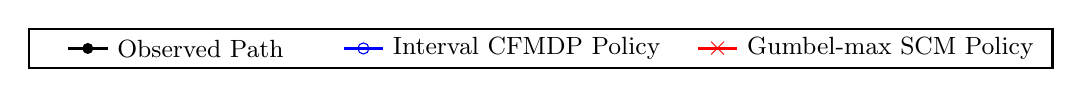
\begin{tikzpicture}[scale=1.0, every node/.style={scale=1.0}]
            \draw[thick, black] (-3, -0.25) rectangle (10, 0.25);
            %
            \draw[black, line width=1pt] (-2.5, 0.0) -- (-2,0.0);
            \fill[black] (-2.25,0.0) circle (2pt); %
            \node[right] at (-2,0.0) {\small Observed Path};
            
            %
            \draw[blue, line width=1pt] (1.0,0.0) -- (1.5,0.0);
            \node[draw=blue, circle, minimum size=4pt, inner sep=0pt] at (1.25,0.0) {}; %
            \node[right] at (1.5,0.0) {\small Interval CFMDP Policy};
            
            %
            \draw[red, line width=1pt] (5.5,0) -- (6,0);
            \node[red] at (5.75,0) {$\boldsymbol{\times}$}; %
            \node[right] at (6,0) {\small Gumbel-max SCM Policy};
        \end{tikzpicture}
    }\\
    %
    \subfigure[\footnotesize Lowest cumulative reward: Interval CFMDP ($312$), Gumbel-max SCM ($312$)]{%
        \resizebox{0.76\columnwidth}{!}{
             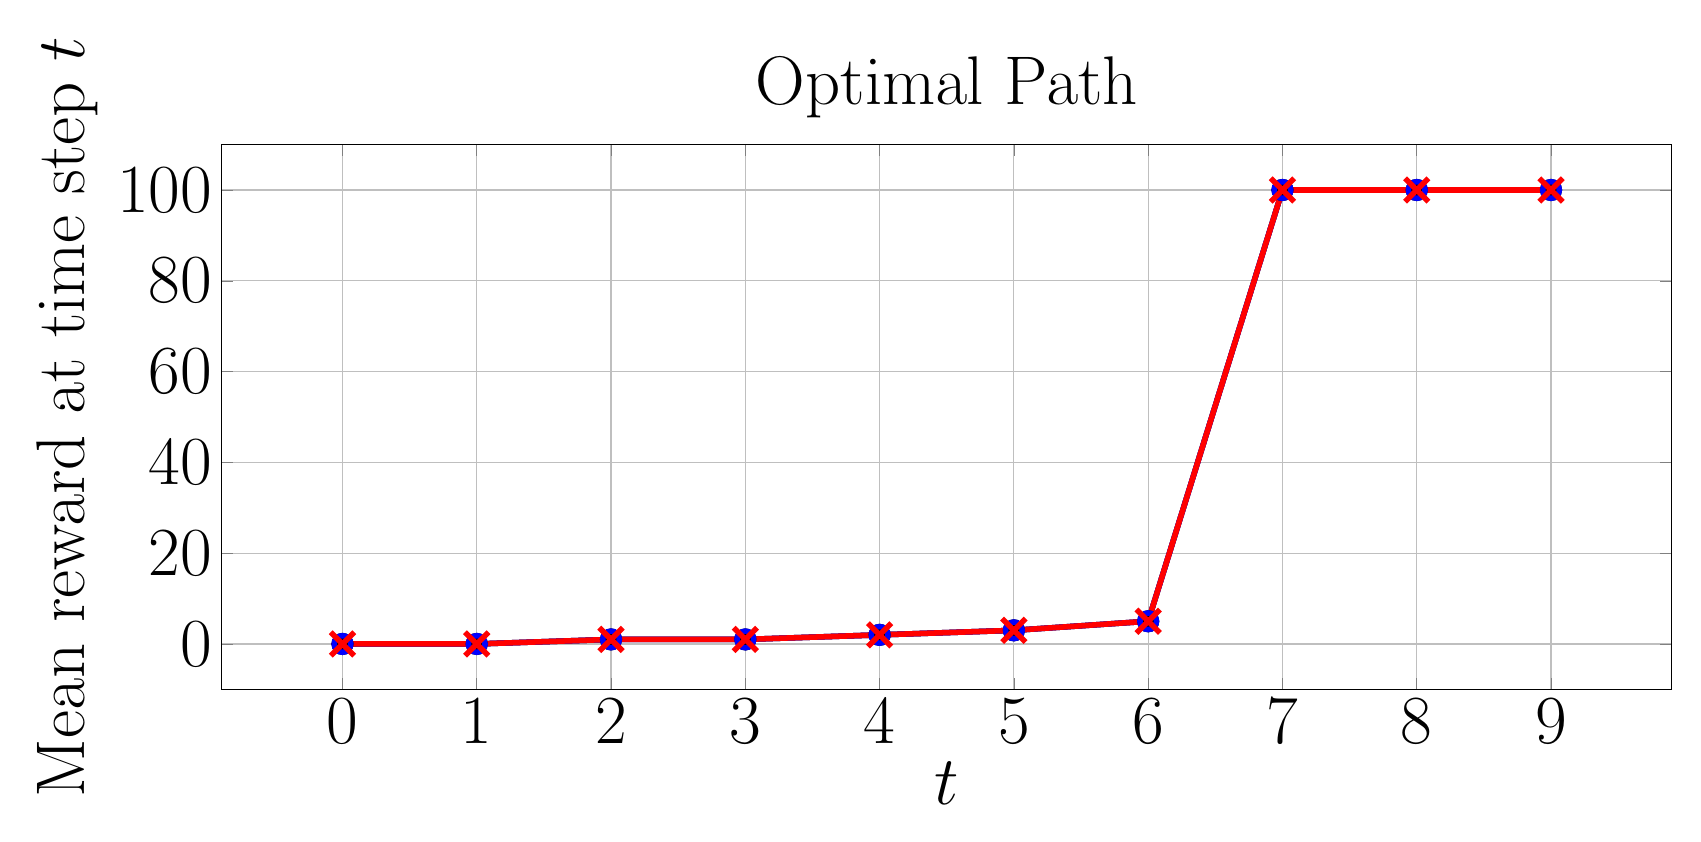
\begin{tikzpicture}
                \begin{axis}[
                    xlabel={$t$},
                    ylabel={Mean reward at time step $t$},
                    title={Optimal Path},
                    grid=both,
                    width=20cm, height=8.5cm,
                    every axis/.style={font=\Huge},
                    %
                ]
                \addplot[
                    color=black, %
                    mark=*, %
                    line width=2pt,
                    mark size=3pt,
                    error bars/.cd,
                    y dir=both, %
                    y explicit, %
                    error bar style={line width=1pt,solid},
                    error mark options={line width=1pt,mark size=4pt,rotate=90}
                ]
                coordinates {
                    (0, 0.0)  +- (0, 0.0)
                    (1, 0.0)  +- (0, 0.0) 
                    (2, 1.0)  +- (0, 0.0) 
                    (3, 1.0)  +- (0, 0.0)
                    (4, 2.0)  +- (0, 0.0)
                    (5, 3.0) +- (0, 0.0)
                    (6, 5.0) +- (0, 0.0)
                    (7, 100.0) +- (0, 0.0)
                    (8, 100.0) +- (0, 0.0)
                    (9, 100.0) +- (0, 0.0)
                };
                %
                \addplot[
                    color=blue, %
                    mark=o, %
                    line width=2pt,
                    mark size=3pt,
                    error bars/.cd,
                    y dir=both, %
                    y explicit, %
                    error bar style={line width=1pt,solid},
                    error mark options={line width=1pt,mark size=4pt,rotate=90}
                ]
                 coordinates {
                    (0, 0.0)  +- (0, 0.0)
                    (1, 0.0)  +- (0, 0.0) 
                    (2, 1.0)  +- (0, 0.0) 
                    (3, 1.0)  +- (0, 0.0)
                    (4, 2.0)  +- (0, 0.0)
                    (5, 3.0) +- (0, 0.0)
                    (6, 5.0) +- (0, 0.0)
                    (7, 100.0) +- (0, 0.0)
                    (8, 100.0) +- (0, 0.0)
                    (9, 100.0) +- (0, 0.0)
                };
                %
                \addplot[
                    color=red, %
                    mark=x, %
                    line width=2pt,
                    mark size=6pt,
                    error bars/.cd,
                    y dir=both, %
                    y explicit, %
                    error bar style={line width=1pt,solid},
                    error mark options={line width=1pt,mark size=4pt,rotate=90}
                ]
                coordinates {
                    (0, 0.0)  +- (0, 0.0)
                    (1, 0.0)  +- (0, 0.0) 
                    (2, 1.0)  +- (0, 0.0) 
                    (3, 1.0)  +- (0, 0.0)
                    (4, 2.0)  +- (0, 0.0)
                    (5, 3.0) +- (0, 0.0)
                    (6, 5.0) +- (0, 0.0)
                    (7, 100.0) +- (0, 0.0)
                    (8, 100.0) +- (0, 0.0)
                    (9, 100.0) +- (0, 0.0)
                };
                \end{axis}
            \end{tikzpicture}
         }
    }
    \hspace{1cm}
    \subfigure[\footnotesize Lowest cumulative reward: Interval CFMDP ($19$), Gumbel-max SCM ($-88$)]{%
         \resizebox{0.76\columnwidth}{!}{
            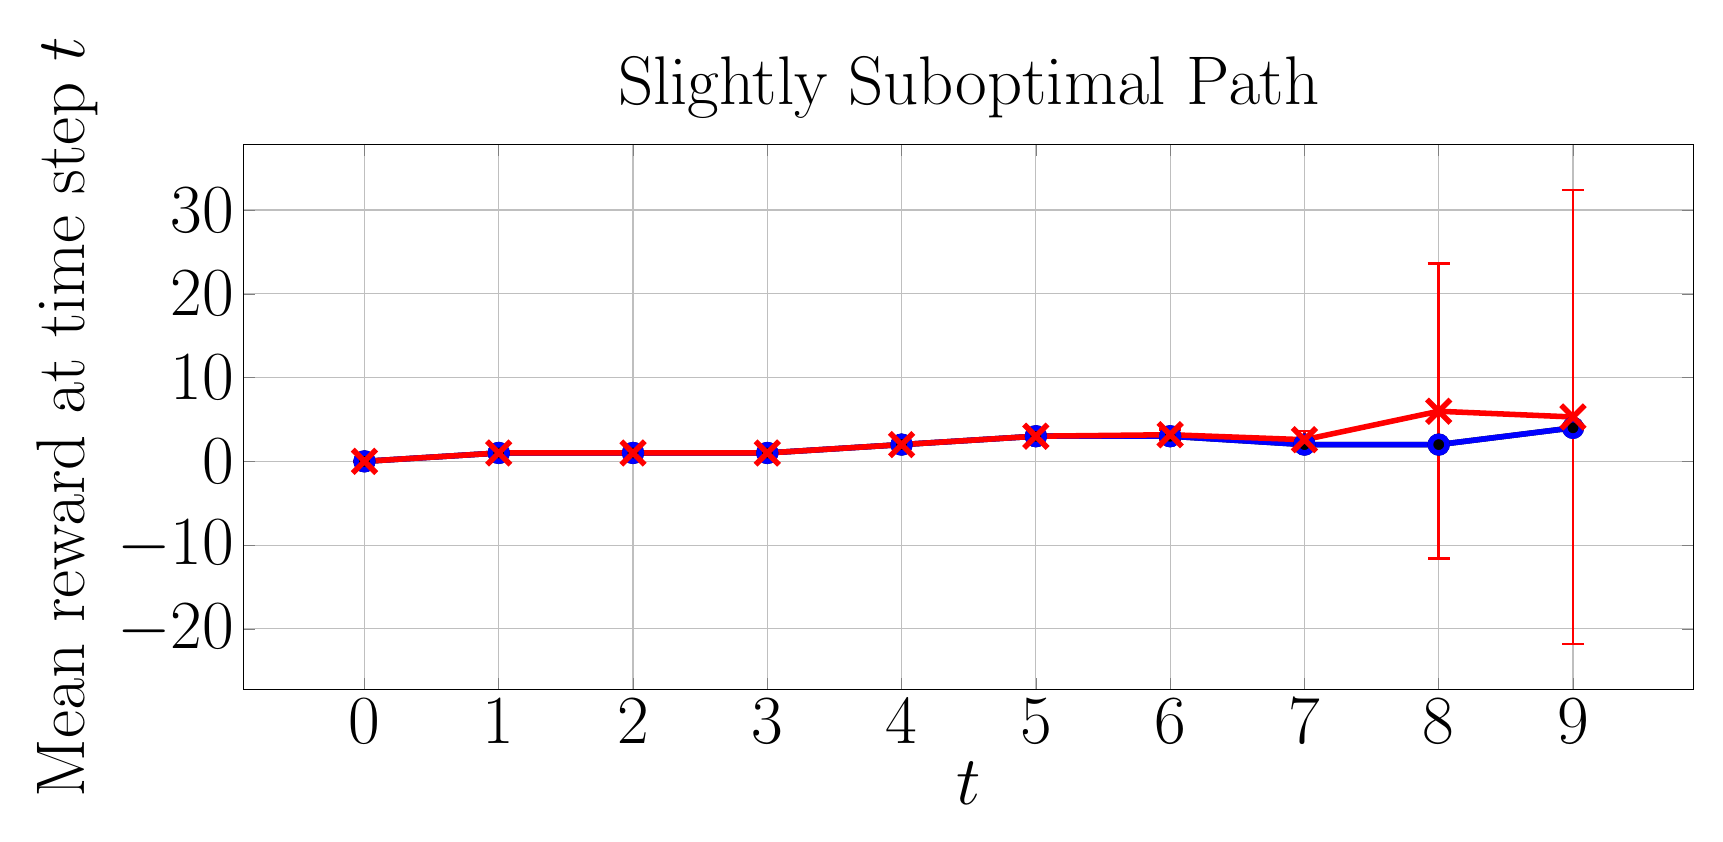
\begin{tikzpicture}
                \begin{axis}[
                    xlabel={$t$},
                    ylabel={Mean reward at time step $t$},
                    title={Slightly Suboptimal Path},
                    grid=both,
                    width=20cm, height=8.5cm,
                    every axis/.style={font=\Huge},
                    %
                ]
                \addplot[
                    color=black, %
                    mark=*, %
                    line width=2pt,
                    mark size=3pt,
                    error bars/.cd,
                    y dir=both, %
                    y explicit, %
                    error bar style={line width=1pt,solid},
                    error mark options={line width=1pt,mark size=4pt,rotate=90}
                ]
              coordinates {
                    (0, 0.0)  +- (0, 0.0)
                    (1, 1.0)  +- (0, 0.0) 
                    (2, 1.0)  +- (0, 0.0) 
                    (3, 1.0)  +- (0, 0.0)
                    (4, 2.0)  +- (0, 0.0)
                    (5, 3.0) +- (0, 0.0)
                    (6, 3.0) +- (0, 0.0)
                    (7, 2.0) +- (0, 0.0)
                    (8, 2.0) +- (0, 0.0)
                    (9, 4.0) +- (0, 0.0)
                };
                %
                \addplot[
                    color=blue, %
                    mark=o, %
                    line width=2pt,
                    mark size=3pt,
                    error bars/.cd,
                    y dir=both, %
                    y explicit, %
                    error bar style={line width=1pt,solid},
                    error mark options={line width=1pt,mark size=4pt,rotate=90}
                ]
              coordinates {
                    (0, 0.0)  +- (0, 0.0)
                    (1, 1.0)  +- (0, 0.0) 
                    (2, 1.0)  +- (0, 0.0) 
                    (3, 1.0)  +- (0, 0.0)
                    (4, 2.0)  +- (0, 0.0)
                    (5, 3.0) +- (0, 0.0)
                    (6, 3.0) +- (0, 0.0)
                    (7, 2.0) +- (0, 0.0)
                    (8, 2.0) +- (0, 0.0)
                    (9, 4.0) +- (0, 0.0)
                };
                %
                \addplot[
                    color=red, %
                    mark=x, %
                    line width=2pt,
                    mark size=6pt,
                    error bars/.cd,
                    y dir=both, %
                    y explicit, %
                    error bar style={line width=1pt,solid},
                    error mark options={line width=1pt,mark size=4pt,rotate=90}
                ]
                coordinates {
                    (0, 0.0)  +- (0, 0.0)
                    (1, 1.0)  +- (0, 0.0) 
                    (2, 1.0)  +- (0, 0.0) 
                    (3, 1.0)  +- (0, 0.0)
                    (4, 2.0)  += (0, 0.0)
                    (5, 3.0)  += (0, 0.0)
                    (6, 3.17847) += (0, 0.62606746) -= (0, 0.62606746)
                    (7, 2.5832885) += (0, 1.04598233) -= (0, 1.04598233)
                    (8, 5.978909) += (0, 17.60137623) -= (0, 17.60137623)
                    (9, 5.297059) += (0, 27.09227512) -= (0, 27.09227512)
                };
                \end{axis}
            \end{tikzpicture}
         }
    }\\[-1.5pt]
    \subfigure[\footnotesize Lowest cumulative reward: Interval CFMDP ($14$), Gumbel-max SCM ($-598$)]{%
         \resizebox{0.76\columnwidth}{!}{
             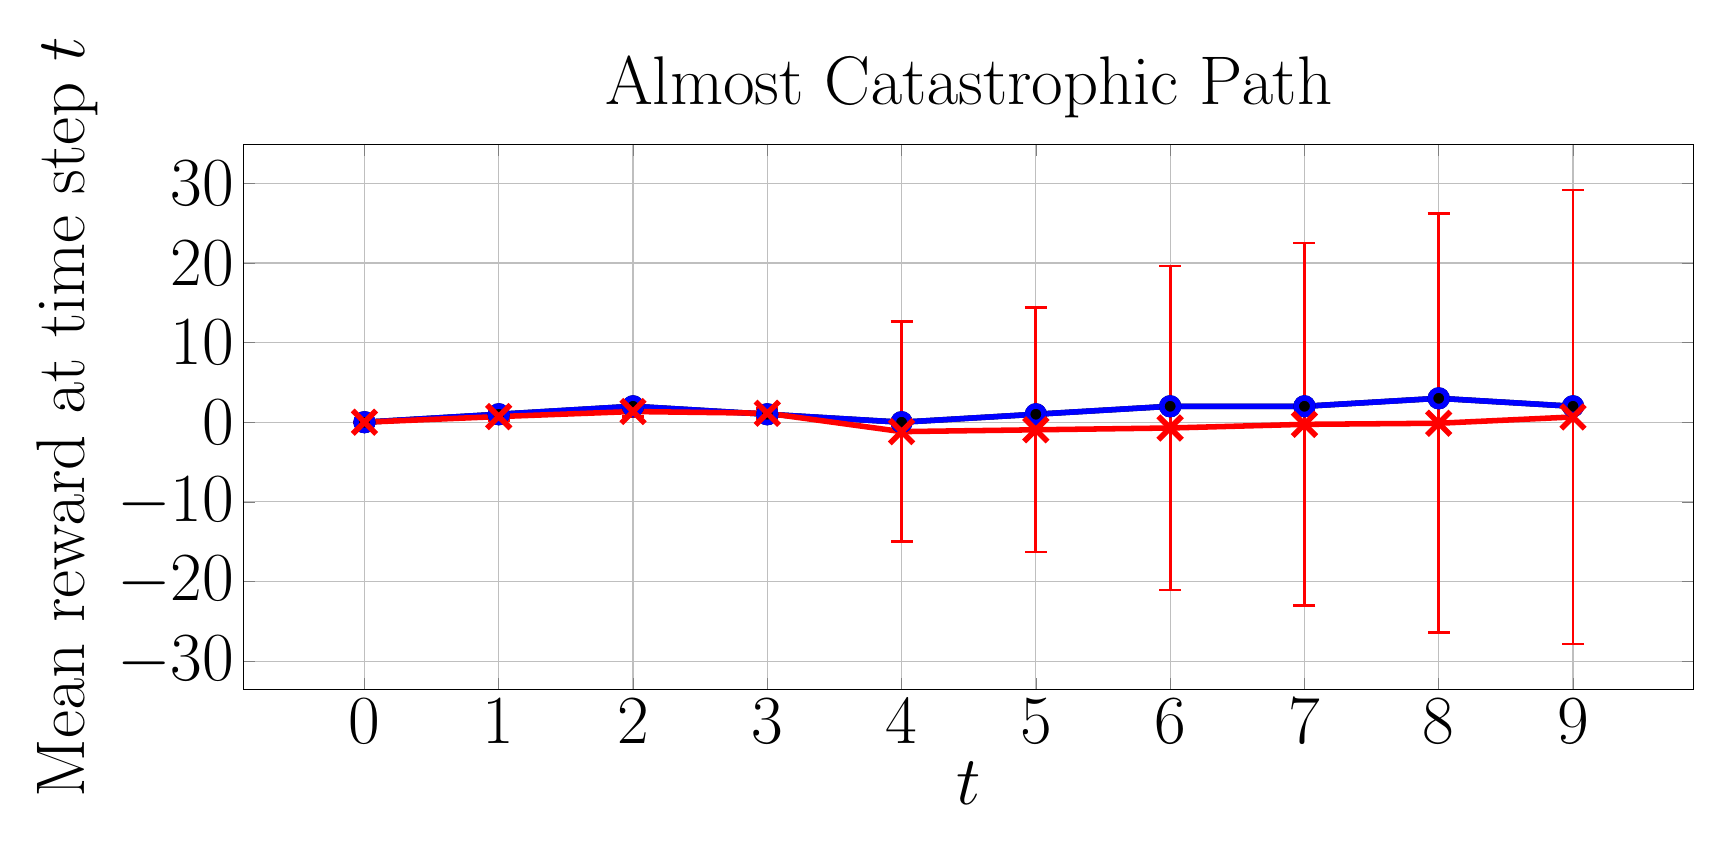
\begin{tikzpicture}
                \begin{axis}[
                    xlabel={$t$},
                    ylabel={Mean reward at time step $t$},
                    title={Almost Catastrophic Path},
                    grid=both,
                    width=20cm, height=8.5cm,
                    every axis/.style={font=\Huge},
                    %
                ]
                \addplot[
                    color=black, %
                    mark=*, %
                    line width=2pt,
                    mark size=3pt,
                    error bars/.cd,
                    y dir=both, %
                    y explicit, %
                    error bar style={line width=1pt,solid},
                    error mark options={line width=1pt,mark size=4pt,rotate=90}
                ]
                coordinates {
                    (0, 0.0)  +- (0, 0.0)
                    (1, 1.0)  +- (0, 0.0) 
                    (2, 2.0)  +- (0, 0.0) 
                    (3, 1.0)  +- (0, 0.0)
                    (4, 0.0)  +- (0, 0.0)
                    (5, 1.0) +- (0, 0.0)
                    (6, 2.0) +- (0, 0.0)
                    (7, 2.0) +- (0, 0.0)
                    (8, 3.0) +- (0, 0.0)
                    (9, 2.0) +- (0, 0.0)
                };
                %
                \addplot[
                    color=blue, %
                    mark=o, %
                    line width=2pt,
                    mark size=3pt,
                    error bars/.cd,
                    y dir=both, %
                    y explicit, %
                    error bar style={line width=1pt,solid},
                    error mark options={line width=1pt,mark size=4pt,rotate=90}
                ]
                coordinates {
                    (0, 0.0)  +- (0, 0.0)
                    (1, 1.0)  +- (0, 0.0) 
                    (2, 2.0)  +- (0, 0.0) 
                    (3, 1.0)  +- (0, 0.0)
                    (4, 0.0)  +- (0, 0.0)
                    (5, 1.0) +- (0, 0.0)
                    (6, 2.0) +- (0, 0.0)
                    (7, 2.0) +- (0, 0.0)
                    (8, 3.0) +- (0, 0.0)
                    (9, 2.0) +- (0, 0.0)
                };
                %
                \addplot[
                    color=red, %
                    mark=x, %
                    line width=2pt,
                    mark size=6pt,
                    error bars/.cd,
                    y dir=both, %
                    y explicit, %
                    error bar style={line width=1pt,solid},
                    error mark options={line width=1pt,mark size=4pt,rotate=90}
                ]
                coordinates {
                    (0, 0.0)  +- (0, 0.0)
                    (1, 0.7065655)  +- (0, 0.4553358) 
                    (2, 1.341673)  +- (0, 0.67091621) 
                    (3, 1.122926)  +- (0, 0.61281824)
                    (4, -1.1821935)  +- (0, 13.82444042)
                    (5, -0.952399)  +- (0, 15.35195457)
                    (6, -0.72672) +- (0, 20.33508414)
                    (7, -0.268983) +- (0, 22.77861454)
                    (8, -0.1310835) +- (0, 26.31013314)
                    (9, 0.65806) +- (0, 28.50670214)
                };
                %
            %
            %
            %
            %
            %
            %
            %
            %
            %
            %
            %
            %
            %
            %
            %
            %
            %
            %
                \end{axis}
            \end{tikzpicture}
         }
    }
    \hspace{1cm}
    \subfigure[\footnotesize Lowest cumulative reward: Interval CFMDP ($-698$), Gumbel-max SCM ($-698$)]{%
         \resizebox{0.76\columnwidth}{!}{
            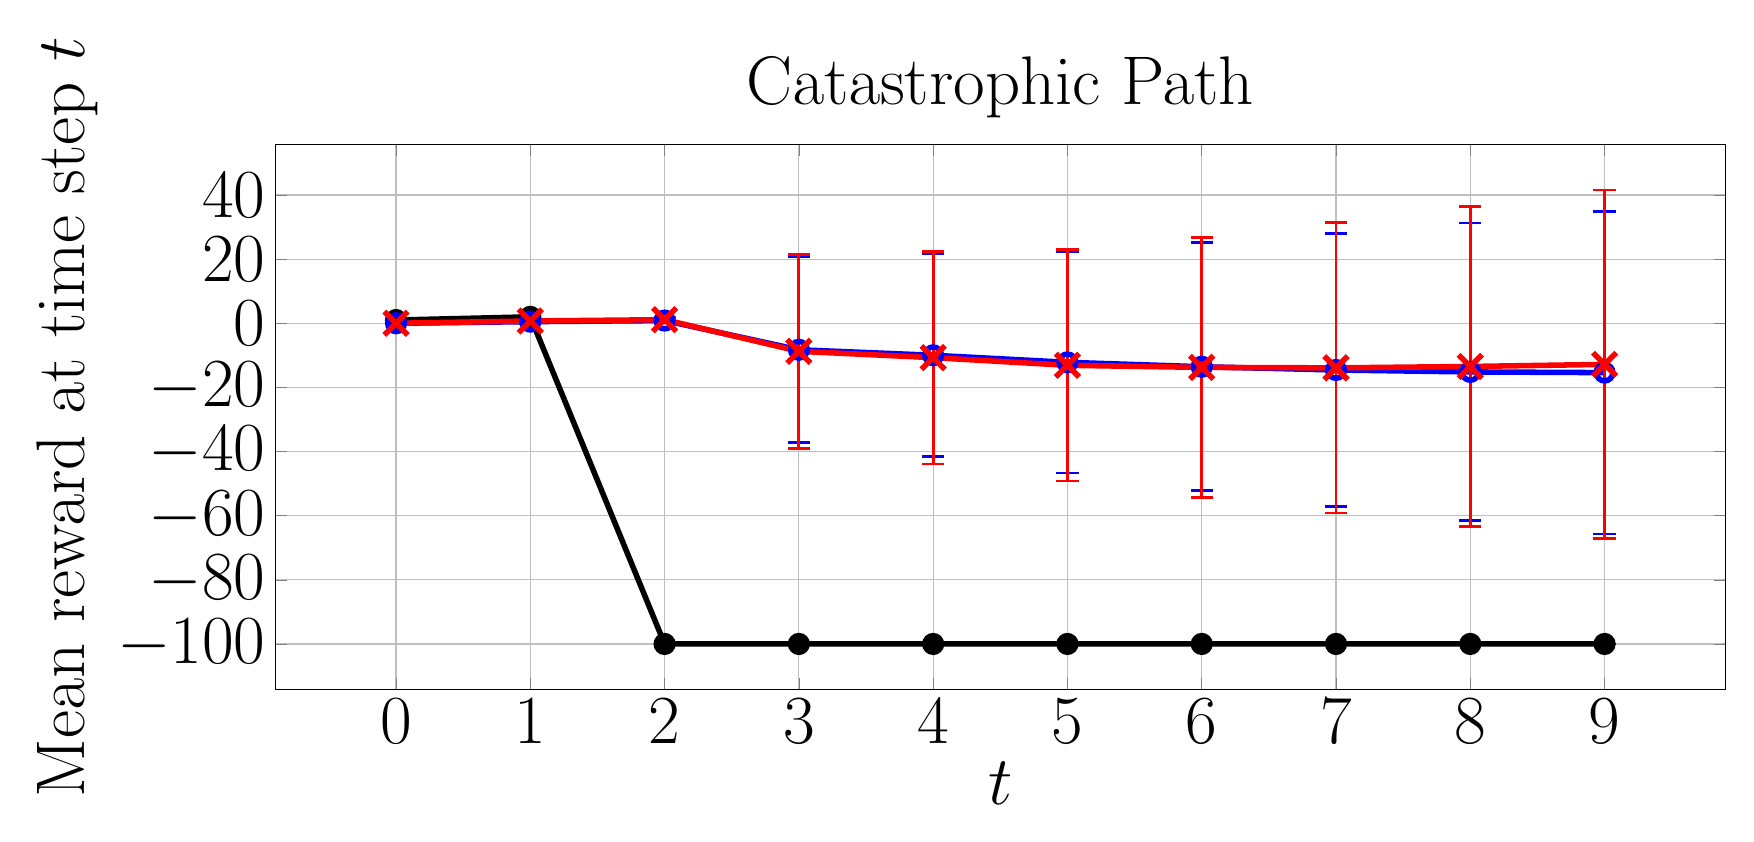
\begin{tikzpicture}
                \begin{axis}[
                    xlabel={$t$},
                    ylabel={Mean reward at time step $t$},
                    title={Catastrophic Path},
                    grid=both,
                    width=20cm, height=8.5cm,
                    every axis/.style={font=\Huge},
                    %
                ]
                \addplot[
                    color=black, %
                    mark=*, %
                    line width=2pt,
                    mark size=3pt,
                    error bars/.cd,
                    y dir=both, %
                    y explicit, %
                    error bar style={line width=1pt,solid},
                    error mark options={line width=1pt,mark size=4pt,rotate=90}
                ]
                coordinates {
                    (0, 1.0)  +- (0, 0.0)
                    (1, 2.0)  +- (0, 0.0) 
                    (2, -100.0)  +- (0, 0.0) 
                    (3, -100.0)  +- (0, 0.0)
                    (4, -100.0)  +- (0, 0.0)
                    (5, -100.0) +- (0, 0.0)
                    (6, -100.0) +- (0, 0.0)
                    (7, -100.0) +- (0, 0.0)
                    (8, -100.0) +- (0, 0.0)
                    (9, -100.0) +- (0, 0.0)
                };
                %
                \addplot[
                    color=blue, %
                    mark=o, %
                    line width=2pt,
                    mark size=3pt,
                    error bars/.cd,
                    y dir=both, %
                    y explicit, %
                    error bar style={line width=1pt,solid},
                    error mark options={line width=1pt,mark size=4pt,rotate=90}
                ]
                coordinates {
                    (0, 0.0)  +- (0, 0.0)
                    (1, 0.504814)  +- (0, 0.49997682) 
                    (2, 0.8439835)  +- (0, 0.76831917) 
                    (3, -8.2709165)  +- (0, 28.93656754)
                    (4, -9.981082)  +- (0, 31.66825363)
                    (5, -12.1776325) +- (0, 34.53463233)
                    (6, -13.556076) +- (0, 38.62845372)
                    (7, -14.574418) +- (0, 42.49603359)
                    (8, -15.1757075) +- (0, 46.41913968)
                    (9, -15.3900395) +- (0, 50.33563368)
                };
                %
                \addplot[
                    color=red, %
                    mark=x, %
                    line width=2pt,
                    mark size=6pt,
                    error bars/.cd,
                    y dir=both, %
                    y explicit, %
                    error bar style={line width=1pt,solid},
                    error mark options={line width=1pt,mark size=4pt,rotate=90}
                ]
                coordinates {
                    (0, 0.0)  +- (0, 0.0)
                    (1, 0.701873)  +- (0, 0.45743556) 
                    (2, 1.1227805)  +- (0, 0.73433129) 
                    (3, -8.7503255)  +- (0, 30.30257976)
                    (4, -10.722092)  +- (0, 33.17618589)
                    (5, -13.10721)  +- (0, 36.0648089)
                    (6, -13.7631645) +- (0, 40.56553451)
                    (7, -13.909043) +- (0, 45.23829402)
                    (8, -13.472517) +- (0, 49.96270296)
                    (9, -12.8278835) +- (0, 54.38618735)
                };
                %
            %
            %
            %
            %
            %
            %
            %
            %
            %
            %
            %
            %
            %
            %
            %
            %
            %
            %
                \end{axis}
            \end{tikzpicture}
         }
    }
    \caption{Average instant reward of CF paths induced by policies on GridWorld $p=0.4$.}
    \label{fig: reward p=0.4}
\end{figure*}

\subsection{Experimental Setup}
To compare policy performance, we measure the average rewards of counterfactual paths induced by our policy and the Gumbel-max policy by uniformly sampling $200$ counterfactual MDPs from the ICFMDP and generating $10,000$ counterfactual paths over each sampled CFMDP. \jl{Since the interval CFMDP depends on the observed path, we select $4$  paths of varying optimality to evaluate how the observed path impacts the performance of both policies: an optimal path, a slightly suboptimal path that could reach the optimal reward with a few changes, a catastrophic path that enters a catastrophic, terminal state with low reward, and an almost catastrophic path that was close to entering a catastrophic state.} When measuring the average probability bound widths and execution time needed to generate the ICFMDPs, we averaged over $20$ randomly generated observed paths
\footnote{Further training details are provided in Appendix \ref{app: training details}, and the code is provided at \href{https://github.com/ddv-lab/robust-cf-inference-in-MDPs}{https://github.com/ddv-lab/robust-cf-inference-in-MDPs}
%
%
.}.

\subsection{GridWorld}
\jl{The GridWorld MDP is a $4 \times 4$ grid where an agent must navigate from the top-left corner to the goal state in the bottom-right corner, avoiding a dangerous terminal state in the centre. At each time step, the agent can move up, down, left, or right, but there is a small probability (controlled by hyper-parameter $p$) of moving in an unintended direction. As the agent nears the goal, the reward for each state increases, culminating in a reward of $+100$ for reaching the goal. Entering the dangerous state results in a penalty of $-100$. We use two versions of GridWorld: a less stochastic version with $p=0.9$ (i.e., $90$\% chance of moving in the chosen direction) and a more stochastic version with $p=0.4$.}

\paragraph{GridWorld ($p=0.9$)}
When $p=0.9$, the counterfactual probability bounds are typically narrow (see Table \ref{tab:nonzero_probs} for average measurements). Consequently, as shown in Figure \ref{fig: reward p=0.9}, both policies are nearly identical and perform similarly well across the optimal, slightly suboptimal, and catastrophic paths.
%
However, for the almost catastrophic path, the interval CFMDP path is more conservative and follows the observed path more closely (as this is where the probability bounds are narrowest), which typically requires one additional step to reach the goal state than the Gumbel-max SCM policy.
%

\paragraph{GridWorld ($p=0.4$)}
\jl{When $p=0.4$, the GridWorld environment becomes more uncertain, increasing the risk of entering the dangerous state even if correct actions are chosen. Thus, as shown in Figure \ref{fig: reward p=0.4}, the interval CFMDP policy adopts a more conservative approach, avoiding deviation from the observed policy if it cannot guarantee higher counterfactual rewards (see the slightly suboptimal and almost catastrophic paths), whereas the Gumbel-max SCM is inconsistent: it can yield higher rewards, but also much lower rewards, reflected in the wide error bars.} For the catastrophic path, both policies must deviate from the observed path to achieve a higher reward and, in this case, perform similarly.
%
%
%
%
\subsection{Sepsis}
The Sepsis MDP \citep{oberst2019counterfactual} simulates trajectories of Sepsis patients. Each state consists of four vital signs (heart rate, blood pressure, oxygen concentration, and glucose levels), categorised as low, normal, or high.
and three treatments that can be toggled on/off at each time step (8 actions in total). Unlike \citet{oberst2019counterfactual}, we scale rewards based on the number of out-of-range vital signs, between $-1000$ (patient dies) and $1000$ (patient discharged). \jl{Like the GridWorld $p=0.4$ experiment, the Sepsis MDP is highly uncertain, as many states are equally likely to lead to optimal and poor outcomes. Thus, as shown in Figure \ref{fig: reward sepsis}, both policies follow the observed optimal and almost catastrophic paths to guarantee rewards are no worse than the observation.} However, improving the catastrophic path requires deviating from the observation. Here, the Gumbel-max SCM policy, on average, performs better than the interval CFMDP policy. But, since both policies have lower bounds clipped at $-1000$, neither policy reliably improves over the observation. In contrast, for the slightly suboptimal path, the interval CFMDP policy performs significantly better, shown by its higher lower bounds. 
Moreover, in these two cases, the worst-case counterfactual path generated by the interval CFMDP policy is better than that of the Gumbel-max SCM policy,
indicating its greater robustness.
%
\begin{figure*}
    \centering
     \resizebox{0.6\textwidth}{!}{
        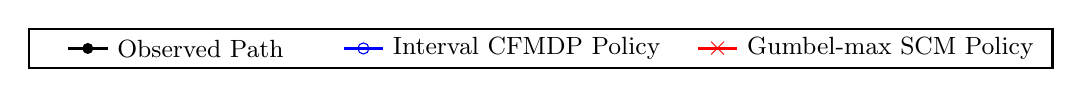
\begin{tikzpicture}[scale=1.0, every node/.style={scale=1.0}]
            \draw[thick, black] (-3, -0.25) rectangle (10, 0.25);
            %
            \draw[black, line width=1pt] (-2.5, 0.0) -- (-2,0.0);
            \fill[black] (-2.25,0.0) circle (2pt); %
            \node[right] at (-2,0.0) {\small Observed Path};
            
            %
            \draw[blue, line width=1pt] (1.0,0.0) -- (1.5,0.0);
            \node[draw=blue, circle, minimum size=4pt, inner sep=0pt] at (1.25,0.0) {}; %
            \node[right] at (1.5,0.0) {\small Interval CFMDP Policy};
            
            %
            \draw[red, line width=1pt] (5.5,0) -- (6,0);
            \node[red] at (5.75,0) {$\boldsymbol{\times}$}; %
            \node[right] at (6,0) {\small Gumbel-max SCM Policy};
        \end{tikzpicture}
    }\\
    \subfigure[\footnotesize Lowest cumulative reward: Interval CFMDP ($8000$), Gumbel-max SCM ($8000$)]{%
         \resizebox{0.76\columnwidth}{!}{
             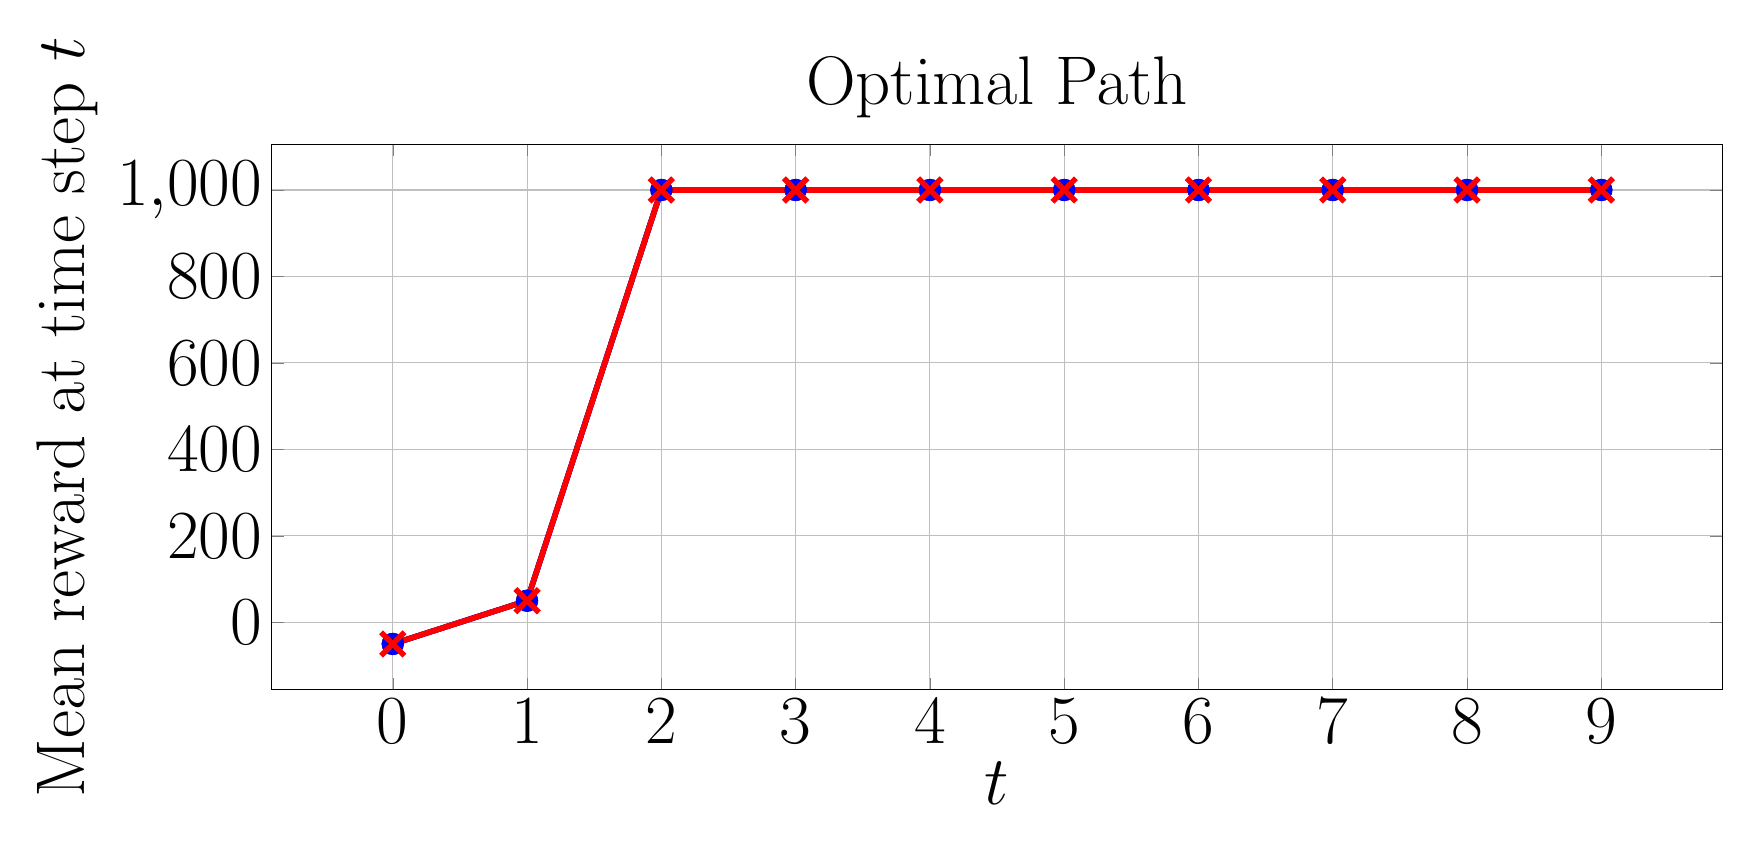
\begin{tikzpicture}
                \begin{axis}[
                    xlabel={$t$},
                    ylabel={Mean reward at time step $t$},
                    title={Optimal Path},
                    grid=both,
                    width=20cm, height=8.5cm,
                    every axis/.style={font=\Huge},
                    %
                ]
                \addplot[
                    color=black, %
                    mark=*, %
                    line width=2pt,
                    mark size=3pt,
                ]
                coordinates {
                    (0, -50.0)
                    (1, 50.0)
                    (2, 1000.0)
                    (3, 1000.0)
                    (4, 1000.0)
                    (5, 1000.0)
                    (6, 1000.0)
                    (7, 1000.0)
                    (8, 1000.0)
                    (9, 1000.0)
                };
                %
                \addplot[
                    color=blue, %
                    mark=o, %
                    line width=2pt,
                    mark size=3pt,
                    error bars/.cd,
                    y dir=both, %
                    y explicit, %
                    error bar style={line width=1pt,solid},
                    error mark options={line width=1pt,mark size=4pt,rotate=90}
                ]
                coordinates {
                    (0, -50.0)  +- (0, 0.0)
                    (1, 50.0)  +- (0, 0.0) 
                    (2, 1000.0)  +- (0, 0.0) 
                    (3, 1000.0)  +- (0, 0.0)
                    (4, 1000.0)  +- (0, 0.0)
                    (5, 1000.0) +- (0, 0.0)
                    (6, 1000.0) +- (0, 0.0)
                    (7, 1000.0) +- (0, 0.0)
                    (8, 1000.0) +- (0, 0.0)
                    (9, 1000.0) +- (0, 0.0)
                };
                %
                \addplot[
                    color=red, %
                    mark=x, %
                    line width=2pt,
                    mark size=6pt,
                    error bars/.cd,
                    y dir=both, %
                    y explicit, %
                    error bar style={line width=1pt,solid},
                    error mark options={line width=1pt,mark size=4pt,rotate=90}
                ]
                coordinates {
                    (0, -50.0)  +- (0, 0.0)
                    (1, 50.0)  +- (0, 0.0) 
                    (2, 1000.0)  +- (0, 0.0) 
                    (3, 1000.0)  +- (0, 0.0)
                    (4, 1000.0)  +- (0, 0.0)
                    (5, 1000.0) +- (0, 0.0)
                    (6, 1000.0) +- (0, 0.0)
                    (7, 1000.0) +- (0, 0.0)
                    (8, 1000.0) +- (0, 0.0)
                    (9, 1000.0) +- (0, 0.0)
                };
                %
                \end{axis}
            \end{tikzpicture}
         }
    }
    \hspace{1cm}
    \subfigure[\footnotesize Lowest cumulative reward: Interval CFMDP ($-5980$), Gumbel-max SCM ($-8000$)]{%
         \resizebox{0.76\columnwidth}{!}{
            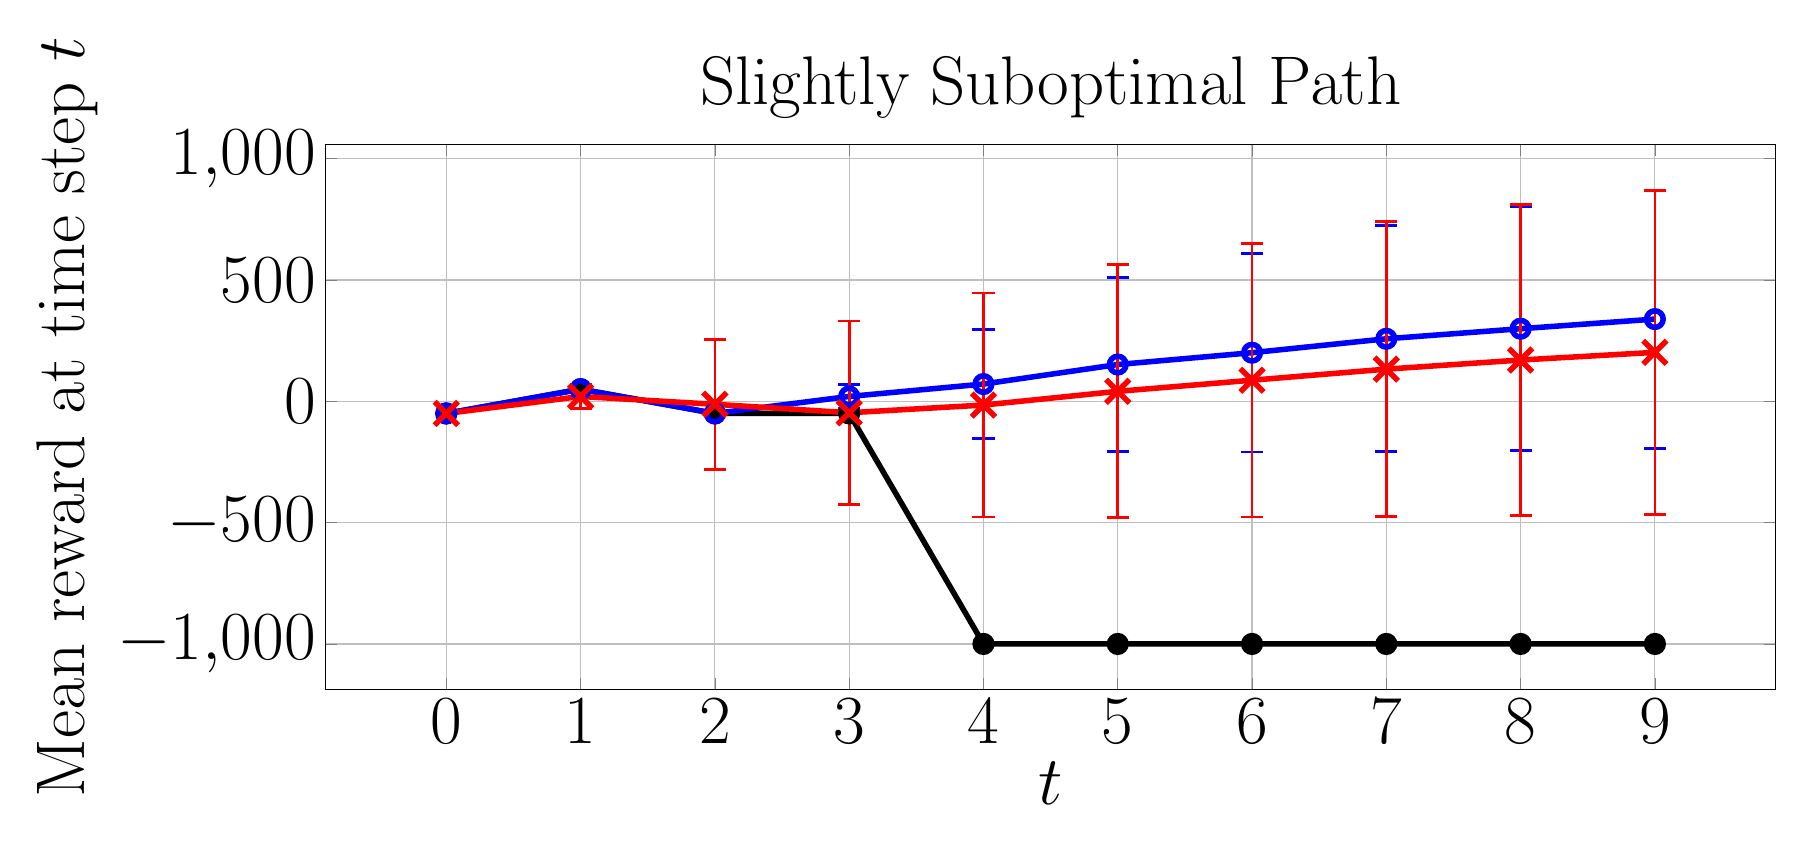
\begin{tikzpicture}
                \begin{axis}[
                    xlabel={$t$},
                    ylabel={Mean reward at time step $t$},
                    title={Slightly Suboptimal Path},
                    grid=both,
                    width=20cm, height=8.5cm,
                    every axis/.style={font=\Huge},
                    %
                ]
               \addplot[
                    color=black, %
                    mark=*, %
                    line width=2pt,
                    mark size=3pt,
                ]
                coordinates {
                    (0, -50.0)
                    (1, 50.0)
                    (2, -50.0)
                    (3, -50.0)
                    (4, -1000.0)
                    (5, -1000.0)
                    (6, -1000.0)
                    (7, -1000.0)
                    (8, -1000.0)
                    (9, -1000.0)
                };
                %
                \addplot[
                    color=blue, %
                    mark=o, %
                    line width=2pt,
                    mark size=3pt,
                    error bars/.cd,
                    y dir=both, %
                    y explicit, %
                    error bar style={line width=1pt,solid},
                    error mark options={line width=1pt,mark size=4pt,rotate=90}
                ]
                coordinates {
                    (0, -50.0)  +- (0, 0.0)
                    (1, 50.0)  +- (0, 0.0) 
                    (2, -50.0)  +- (0, 0.0) 
                    (3, 20.0631)  +- (0, 49.97539413)
                    (4, 71.206585)  +- (0, 226.02033693)
                    (5, 151.60797) +- (0, 359.23292559)
                    (6, 200.40593) +- (0, 408.86185176)
                    (7, 257.77948) +- (0, 466.10372804)
                    (8, 299.237465) +- (0, 501.82579506)
                    (9, 338.9129) +- (0, 532.06124996)
                };
                %
                \addplot[
                    color=red, %
                    mark=x, %
                    line width=2pt,
                    mark size=6pt,
                    error bars/.cd,
                    y dir=both, %
                    y explicit, %
                    error bar style={line width=1pt,solid},
                    error mark options={line width=1pt,mark size=4pt,rotate=90}
                ]
                coordinates {
                    (0, -50.0)  +- (0, 0.0)
                    (1, 20.00736)  +- (0, 49.99786741) 
                    (2, -12.282865)  +- (0, 267.598755) 
                    (3, -47.125995)  +- (0, 378.41755832)
                    (4, -15.381965)  +- (0, 461.77616558)
                    (5, 41.15459) +- (0, 521.53189262)
                    (6, 87.01595) +- (0, 564.22243126 )
                    (7, 132.62376) +- (0, 607.31338037)
                    (8, 170.168145) +- (0, 641.48013693)
                    (9, 201.813135) +- (0, 667.29441777)
                };
                %
                %
                %
                %
                %
                %
                %
                %
                %
                %
                %
                %
                %
                %
                %
                %
                %
                %
                %
                \end{axis}
            \end{tikzpicture}
         }
    }\\[-1.5pt]
    \subfigure[\footnotesize Lowest cumulative reward: Interval CFMDP ($100$), Gumbel-max SCM ($100$)]{%
         \resizebox{0.76\columnwidth}{!}{
             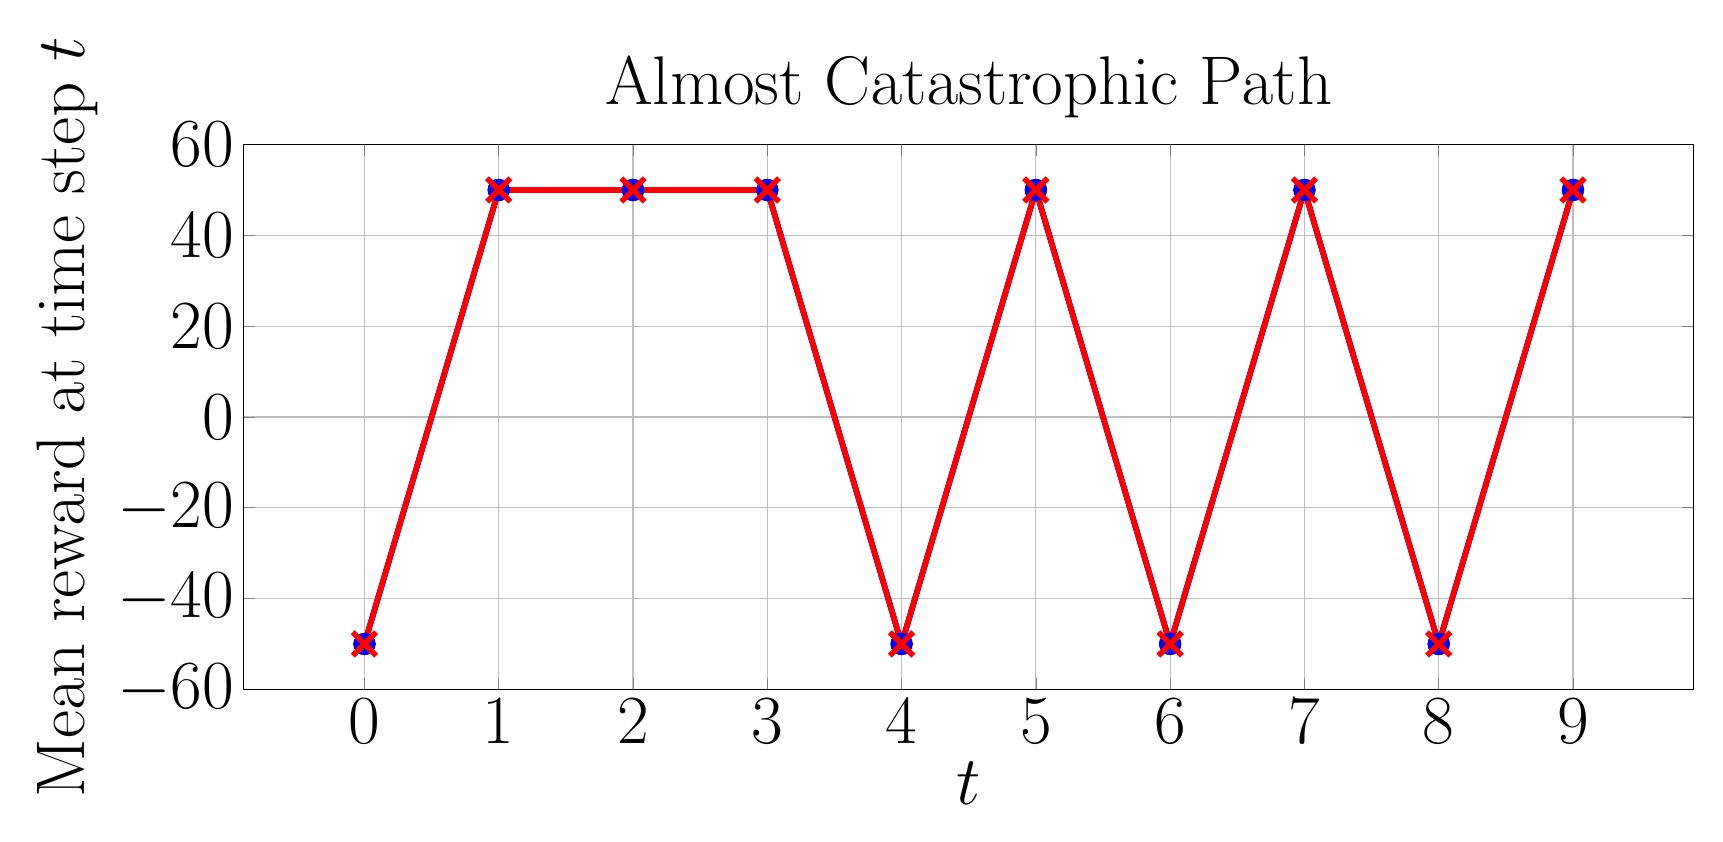
\begin{tikzpicture}
                \begin{axis}[
                    xlabel={$t$},
                    ylabel={Mean reward at time step $t$},
                    title={Almost Catastrophic Path},
                    grid=both,
                    every axis/.style={font=\Huge},
                    width=20cm, height=8.5cm,
                    %
                ]
               \addplot[
                    color=black, %
                    mark=*, %
                    line width=2pt,
                    mark size=3pt,
                ]
                coordinates {
                    (0, -50.0)
                    (1, 50.0)
                    (2, 50.0)
                    (3, 50.0)
                    (4, -50.0)
                    (5, 50.0)
                    (6, -50.0)
                    (7, 50.0)
                    (8, -50.0)
                    (9, 50.0)
                };
                %
                %
                \addplot[
                    color=blue, %
                    mark=o, %
                    line width=2pt,
                    mark size=3pt,
                    error bars/.cd,
                    y dir=both, %
                    y explicit, %
                    error bar style={line width=1pt,solid},
                    error mark options={line width=1pt,mark size=4pt,rotate=90}
                ]
                coordinates {
                    (0, -50.0)  +- (0, 0.0)
                    (1, 50.0)  +- (0, 0.0) 
                    (2, 50.0)  +- (0, 0.0) 
                    (3, 50.0)  +- (0, 0.0)
                    (4, -50.0)  +- (0, 0.0)
                    (5, 50.0) +- (0, 0.0)
                    (6, -50.0) +- (0, 0.0)
                    (7, 50.0) +- (0, 0.0)
                    (8, -50.0) +- (0, 0.0)
                    (9, 50.0) +- (0, 0.0)
                };
                %
                \addplot[
                    color=red, %
                    mark=x, %
                    line width=2pt,
                    mark size=6pt,
                    error bars/.cd,
                    y dir=both, %
                    y explicit, %
                    error bar style={line width=1pt,solid},
                    error mark options={line width=1pt,mark size=4pt,rotate=90}
                ]
                coordinates {
                    (0, -50.0)  +- (0, 0.0)
                    (1, 50.0)  +- (0, 0.0) 
                    (2, 50.0)  +- (0, 0.0) 
                    (3, 50.0)  +- (0, 0.0)
                    (4, -50.0)  +- (0, 0.0)
                    (5, 50.0) +- (0, 0.0)
                    (6, -50.0) +- (0, 0.0)
                    (7, 50.0) +- (0, 0.0)
                    (8, -50.0) +- (0, 0.0)
                    (9, 50.0) +- (0, 0.0)
                };
                %
                %
                %
                %
                %
                %
                %
                %
                %
                %
                %
                %
                %
                %
                %
                %
                %
                %
                %
                \end{axis}
            \end{tikzpicture}
         }
    }
    \hspace{1cm}
    \subfigure[\footnotesize Lowest cumulative reward: Interval CFMDP ($-7150$), Gumbel-max SCM ($-9050$)]{%
         \resizebox{0.76\columnwidth}{!}{
            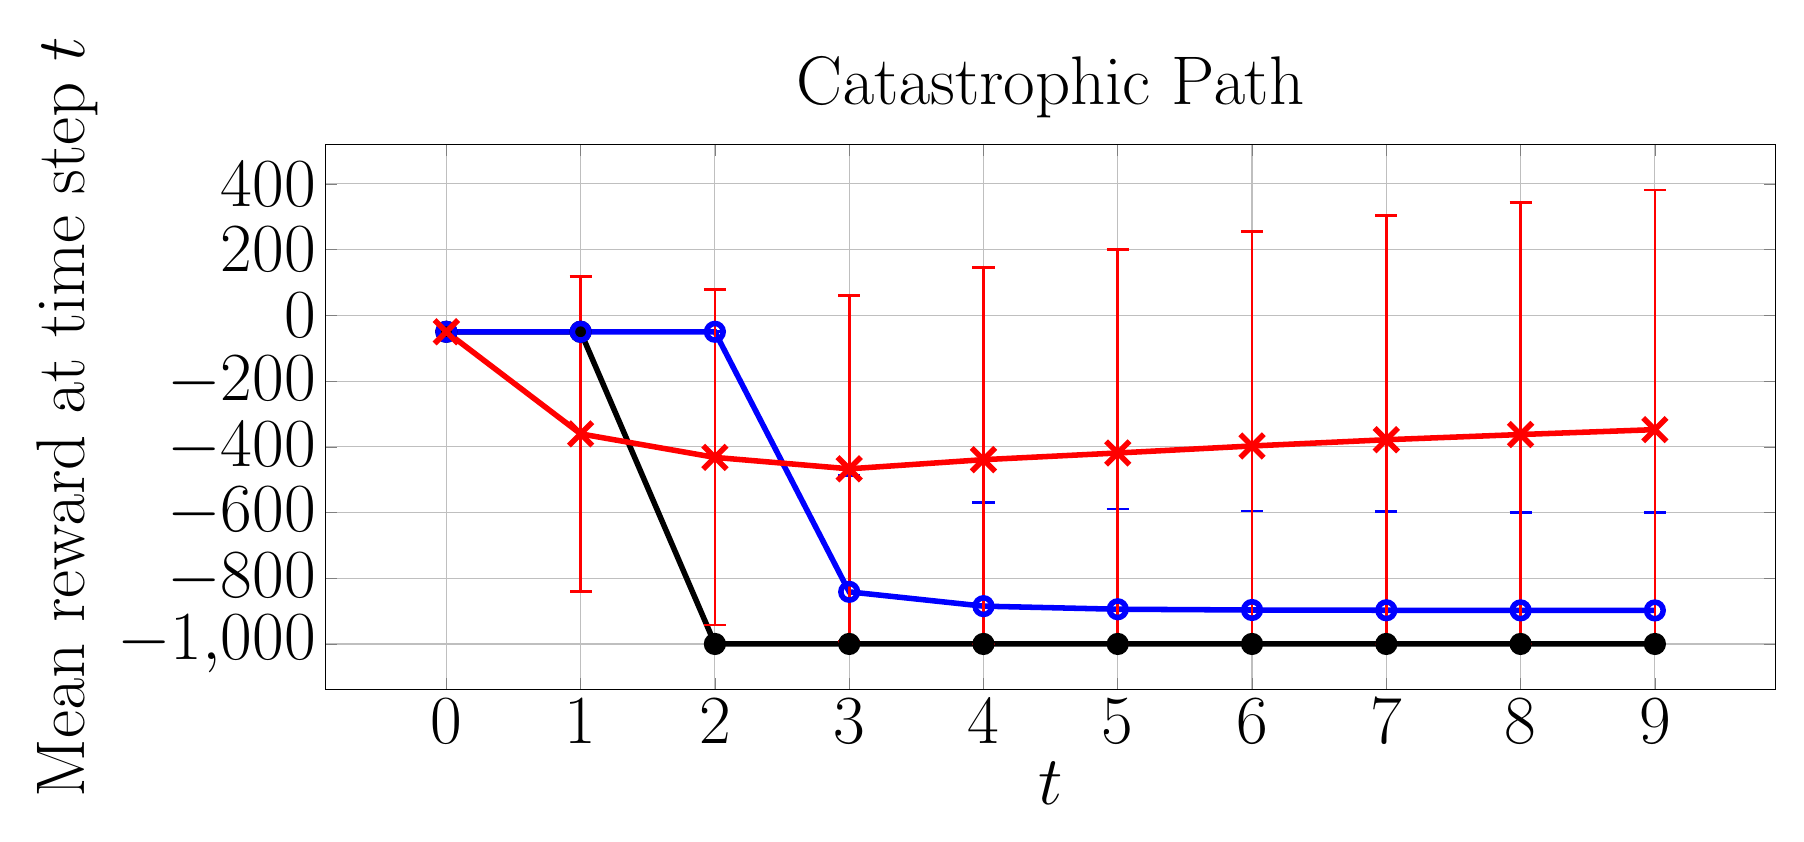
\begin{tikzpicture}
                \begin{axis}[
                    xlabel={$t$},
                    ylabel={Mean reward at time step $t$},
                    title={Catastrophic Path},
                    grid=both,
                    width=20cm, height=8.5cm,
                    every axis/.style={font=\Huge},
                    %
                ]
               \addplot[
                    color=black, %
                    mark=*, %
                    line width=2pt,
                    mark size=3pt,
                ]
                coordinates {
                    (0, -50.0)
                    (1, -50.0)
                    (2, -1000.0)
                    (3, -1000.0)
                    (4, -1000.0)
                    (5, -1000.0)
                    (6, -1000.0)
                    (7, -1000.0)
                    (8, -1000.0)
                    (9, -1000.0)
                };
                %
                %
                \addplot[
                    color=blue, %
                    mark=o, %
                    line width=2pt,
                    mark size=3pt,
                    error bars/.cd,
                    y dir=both, %
                    y explicit, %
                    error bar style={line width=1pt,solid},
                    error mark options={line width=1pt,mark size=4pt,rotate=90}
                ]
                coordinates {
                    (0, -50.0)  +- (0, 0.0)
                    (1, -50.0)  +- (0, 0.0) 
                    (2, -50.0)  +- (0, 0.0) 
                    (3, -841.440725)  += (0, 354.24605512) -= (0, 158.559275)
                    (4, -884.98225)  += (0, 315.37519669) -= (0, 115.01775)
                    (5, -894.330425) += (0, 304.88572805) -= (0, 105.669575)
                    (6, -896.696175) += (0, 301.19954514) -= (0, 103.303825)
                    (7, -897.4635) += (0, 299.61791279) -= (0, 102.5365)
                    (8, -897.77595) += (0, 298.80392585) -= (0, 102.22405)
                    (9, -897.942975) += (0, 298.32920557) -= (0, 102.057025)
                };
                %
                \addplot[
                    color=red, %
                    mark=x, %
                    line width=2pt,
                    mark size=6pt,
                    error bars/.cd,
                    y dir=both, %
                    y explicit, %
                    error bar style={line width=1pt,solid},
                    error mark options={line width=1pt,mark size=4pt,rotate=90}
                ]
            coordinates {
                    (0, -50.0)  +- (0, 0.0)
                    (1, -360.675265)  +- (0, 479.39812699) 
                    (2, -432.27629)  +- (0, 510.38620897) 
                    (3, -467.029545)  += (0, 526.36009628) -= (0, 526.36009628)
                    (4, -439.17429)  += (0, 583.96638919) -= (0, 560.82571)
                    (5, -418.82704) += (0, 618.43027478) -= (0, 581.17296)
                    (6, -397.464895) += (0, 652.67322574) -= (0, 602.535105)
                    (7, -378.49052) += (0, 682.85407033) -= (0, 621.50948)
                    (8, -362.654195) += (0, 707.01412023) -= (0, 637.345805)
                    (9, -347.737935) += (0, 729.29076479) -= (0, 652.262065)
                };
                %
                %
                %
                %
                %
                %
                %
                %
                %
                %
                %
                %
                %
                %
                %
                %
                %
                %
                %
                \end{axis}
            \end{tikzpicture}
         }
    }
    \caption{Average instant reward of CF paths induced by policies on Sepsis.}
    \label{fig: reward sepsis}
\end{figure*}

%
%
%
\subsection{Interval CFMDP Bounds}
%
%
Table \ref{tab:nonzero_probs} presents the mean counterfactual probability bound widths (excluding transitions where the upper bound is $0$) for each MDP, averaged over 20 observed paths. We compare the bounds under counterfactual stability (CS) and monotonicity (M) assumptions, CS alone, and no assumptions. This shows that the assumptions marginally reduce the bound widths, indicating the assumptions tighten the bounds without excluding too many causal models, as intended.
\renewcommand{\arraystretch}{1}

\begin{table}
\centering
\caption{Mean width of counterfactual probability bounds}
\resizebox{0.8\columnwidth}{!}{%
\begin{tabular}{|c|c|c|c|}
\hline
\multirow{2}{*}{\textbf{Environment}} & \multicolumn{3}{c|}{\textbf{Assumptions}} \\ \cline{2-4}
 & \textbf{CS + M} & \textbf{CS} & \textbf{None\tablefootnote{\jl{Equivalent to \citet{li2024probabilities}'s bounds (see Section \ref{sec: equivalence with Li}).}}} \\ \hline
\textbf{GridWorld} ($p=0.9$) & 0.0817 & 0.0977 & 0.100 \\ \hline
\textbf{GridWorld} ($p=0.4$) & 0.552  & 0.638  & 0.646 \\ \hline
\textbf{Sepsis} & 0.138 & 0.140 & 0.140 \\ \hline
\end{tabular}
}
\label{tab:nonzero_probs}
\end{table}


\subsection{Execution Times}
Table \ref{tab: times} compares the average time needed to generate the interval CFMDP vs.\ the Gumbel-max SCM CFMDP for 20 observations.
The GridWorld algorithms were run single-threaded, while the Sepsis experiments were run in parallel.
Generating the interval CFMDP is significantly faster as it uses exact analytical bounds, whereas the Gumbel-max CFMDP requires sampling from the Gumbel distribution to estimate counterfactual transition probabilities. \jl{Since constructing the counterfactual MDP models is the main bottleneck in both approaches, ours is more efficient overall and suitable for larger MDPs.}
\begin{table}
\centering
\caption{Mean execution time to generate CFMDPs}
\resizebox{0.99\columnwidth}{!}{%
\begin{tabular}{|c|c|c|}
\hline
\multirow{2}{*}{\textbf{Environment}} & \multicolumn{2}{c|}{\textbf{Mean Execution Time (s)}} \\ \cline{2-3} 
                                      & \textbf{Interval CFMDP} & \textbf{Gumbel-max CFMDP} \\ \hline
\textbf{GridWorld ($p=0.9$) }                  & 0.261                   & 56.1                      \\ \hline
\textbf{GridWorld ($p=0.4$)  }                 & 0.336                   & 54.5                      \\ \hline
\textbf{Sepsis}                                 & 688                     & 2940                      \\ \hline
\end{tabular}%
}
\label{tab: times}
\end{table}

\section{Discussion of Assumptions}\label{sec:discussion}
In this paper, we have made several assumptions for the sake of clarity and simplicity. In this section, we discuss the rationale behind these assumptions, the extent to which these assumptions hold in practice, and the consequences for our protocol when these assumptions hold.

\subsection{Assumptions on the Demand}

There are two simplifying assumptions we make about the demand. First, we assume the demand at any time is relatively small compared to the channel capacities. Second, we take the demand to be constant over time. We elaborate upon both these points below.

\paragraph{Small demands} The assumption that demands are small relative to channel capacities is made precise in \eqref{eq:large_capacity_assumption}. This assumption simplifies two major aspects of our protocol. First, it largely removes congestion from consideration. In \eqref{eq:primal_problem}, there is no constraint ensuring that total flow in both directions stays below capacity--this is always met. Consequently, there is no Lagrange multiplier for congestion and no congestion pricing; only imbalance penalties apply. In contrast, protocols in \cite{sivaraman2020high, varma2021throughput, wang2024fence} include congestion fees due to explicit congestion constraints. Second, the bound \eqref{eq:large_capacity_assumption} ensures that as long as channels remain balanced, the network can always meet demand, no matter how the demand is routed. Since channels can rebalance when necessary, they never drop transactions. This allows prices and flows to adjust as per the equations in \eqref{eq:algorithm}, which makes it easier to prove the protocol's convergence guarantees. This also preserves the key property that a channel's price remains proportional to net money flow through it.

In practice, payment channel networks are used most often for micro-payments, for which on-chain transactions are prohibitively expensive; large transactions typically take place directly on the blockchain. For example, according to \cite{river2023lightning}, the average channel capacity is roughly $0.1$ BTC ($5,000$ BTC distributed over $50,000$ channels), while the average transaction amount is less than $0.0004$ BTC ($44.7k$ satoshis). Thus, the small demand assumption is not too unrealistic. Additionally, the occasional large transaction can be treated as a sequence of smaller transactions by breaking it into packets and executing each packet serially (as done by \cite{sivaraman2020high}).
Lastly, a good path discovery process that favors large capacity channels over small capacity ones can help ensure that the bound in \eqref{eq:large_capacity_assumption} holds.

\paragraph{Constant demands} 
In this work, we assume that any transacting pair of nodes have a steady transaction demand between them (see Section \ref{sec:transaction_requests}). Making this assumption is necessary to obtain the kind of guarantees that we have presented in this paper. Unless the demand is steady, it is unreasonable to expect that the flows converge to a steady value. Weaker assumptions on the demand lead to weaker guarantees. For example, with the more general setting of stochastic, but i.i.d. demand between any two nodes, \cite{varma2021throughput} shows that the channel queue lengths are bounded in expectation. If the demand can be arbitrary, then it is very hard to get any meaningful performance guarantees; \cite{wang2024fence} shows that even for a single bidirectional channel, the competitive ratio is infinite. Indeed, because a PCN is a decentralized system and decisions must be made based on local information alone, it is difficult for the network to find the optimal detailed balance flow at every time step with a time-varying demand.  With a steady demand, the network can discover the optimal flows in a reasonably short time, as our work shows.

We view the constant demand assumption as an approximation for a more general demand process that could be piece-wise constant, stochastic, or both (see simulations in Figure \ref{fig:five_nodes_variable_demand}).
We believe it should be possible to merge ideas from our work and \cite{varma2021throughput} to provide guarantees in a setting with random demands with arbitrary means. We leave this for future work. In addition, our work suggests that a reasonable method of handling stochastic demands is to queue the transaction requests \textit{at the source node} itself. This queuing action should be viewed in conjunction with flow-control. Indeed, a temporarily high unidirectional demand would raise prices for the sender, incentivizing the sender to stop sending the transactions. If the sender queues the transactions, they can send them later when prices drop. This form of queuing does not require any overhaul of the basic PCN infrastructure and is therefore simpler to implement than per-channel queues as suggested by \cite{sivaraman2020high} and \cite{varma2021throughput}.

\subsection{The Incentive of Channels}
The actions of the channels as prescribed by the DEBT control protocol can be summarized as follows. Channels adjust their prices in proportion to the net flow through them. They rebalance themselves whenever necessary and execute any transaction request that has been made of them. We discuss both these aspects below.

\paragraph{On Prices}
In this work, the exclusive role of channel prices is to ensure that the flows through each channel remains balanced. In practice, it would be important to include other components in a channel's price/fee as well: a congestion price  and an incentive price. The congestion price, as suggested by \cite{varma2021throughput}, would depend on the total flow of transactions through the channel, and would incentivize nodes to balance the load over different paths. The incentive price, which is commonly used in practice \cite{river2023lightning}, is necessary to provide channels with an incentive to serve as an intermediary for different channels. In practice, we expect both these components to be smaller than the imbalance price. Consequently, we expect the behavior of our protocol to be similar to our theoretical results even with these additional prices.

A key aspect of our protocol is that channel fees are allowed to be negative. Although the original Lightning network whitepaper \cite{poon2016bitcoin} suggests that negative channel prices may be a good solution to promote rebalancing, the idea of negative prices in not very popular in the literature. To our knowledge, the only prior work with this feature is \cite{varma2021throughput}. Indeed, in papers such as \cite{van2021merchant} and \cite{wang2024fence}, the price function is explicitly modified such that the channel price is never negative. The results of our paper show the benefits of negative prices. For one, in steady state, equal flows in both directions ensure that a channel doesn't loose any money (the other price components mentioned above ensure that the channel will only gain money). More importantly, negative prices are important to ensure that the protocol selectively stifles acyclic flows while allowing circulations to flow. Indeed, in the example of Section \ref{sec:flow_control_example}, the flows between nodes $A$ and $C$ are left on only because the large positive price over one channel is canceled by the corresponding negative price over the other channel, leading to a net zero price.

Lastly, observe that in the DEBT control protocol, the price charged by a channel does not depend on its capacity. This is a natural consequence of the price being the Lagrange multiplier for the net-zero flow constraint, which also does not depend on the channel capacity. In contrast, in many other works, the imbalance price is normalized by the channel capacity \cite{ren2018optimal, lin2020funds, wang2024fence}; this is shown to work well in practice. The rationale for such a price structure is explained well in \cite{wang2024fence}, where this fee is derived with the aim of always maintaining some balance (liquidity) at each end of every channel. This is a reasonable aim if a channel is to never rebalance itself; the experiments of the aforementioned papers are conducted in such a regime. In this work, however, we allow the channels to rebalance themselves a few times in order to settle on a detailed balance flow. This is because our focus is on the long-term steady state performance of the protocol. This difference in perspective also shows up in how the price depends on the channel imbalance. \cite{lin2020funds} and \cite{wang2024fence} advocate for strictly convex prices whereas this work and \cite{varma2021throughput} propose linear prices.

\paragraph{On Rebalancing} 
Recall that the DEBT control protocol ensures that the flows in the network converge to a detailed balance flow, which can be sustained perpetually without any rebalancing. However, during the transient phase (before convergence), channels may have to perform on-chain rebalancing a few times. Since rebalancing is an expensive operation, it is worthwhile discussing methods by which channels can reduce the extent of rebalancing. One option for the channels to reduce the extent of rebalancing is to increase their capacity; however, this comes at the cost of locking in more capital. Each channel can decide for itself the optimum amount of capital to lock in. Another option, which we discuss in Section \ref{sec:five_node}, is for channels to increase the rate $\gamma$ at which they adjust prices. 

Ultimately, whether or not it is beneficial for a channel to rebalance depends on the time-horizon under consideration. Our protocol is based on the assumption that the demand remains steady for a long period of time. If this is indeed the case, it would be worthwhile for a channel to rebalance itself as it can make up this cost through the incentive fees gained from the flow of transactions through it in steady state. If a channel chooses not to rebalance itself, however, there is a risk of being trapped in a deadlock, which is suboptimal for not only the nodes but also the channel.

\section{Conclusion}
This work presents DEBT control: a protocol for payment channel networks that uses source routing and flow control based on channel prices. The protocol is derived by posing a network utility maximization problem and analyzing its dual minimization. It is shown that under steady demands, the protocol guides the network to an optimal, sustainable point. Simulations show its robustness to demand variations. The work demonstrates that simple protocols with strong theoretical guarantees are possible for PCNs and we hope it inspires further theoretical research in this direction.
\section{Conclusion}
In this work, we propose a simple yet effective approach, called SMILE, for graph few-shot learning with fewer tasks. Specifically, we introduce a novel dual-level mixup strategy, including within-task and across-task mixup, for enriching the diversity of nodes within each task and the diversity of tasks. Also, we incorporate the degree-based prior information to learn expressive node embeddings. Theoretically, we prove that SMILE effectively enhances the model's generalization performance. Empirically, we conduct extensive experiments on multiple benchmarks and the results suggest that SMILE significantly outperforms other baselines, including both in-domain and cross-domain few-shot settings.

\begin{acks}
We are grateful to Dongyang Zhong, Lin-Ping Yuan, Liwenhan Xie, Rui Sheng, and Chenyang Zhang for their kind help.
This work is partially supported by the Hong Kong RGC GRF grant 16210722.
\end{acks}

\bibliographystyle{ACM-Reference-Format}
\bibliography{references}

\end{document}
\endinput
%%
%% End of file `sample-manuscript.tex'.
